\documentclass{article}

\usepackage{amsmath}
\usepackage{amssymb}
\usepackage{fullpage}
\usepackage{bm}
\usepackage{natbib}
\usepackage{tikz}
\usepackage{pgfplots}
\usepackage{fixltx2e}
\usepackage{dblfloatfix}
\usepackage{gensymb}

\usepackage{graphicx}
\usepackage{subfigure} 
\usepackage{hyperref}

\newcommand{\argmax}{ \operatorname*{arg \max}}
\newcommand{\argmin}{ \operatorname*{arg \min}} 
\newcommand{\x}{\mathbf{x}} 
\newcommand{\pair}{(\x,\x')} 
\newcommand{\param}{\bm{\theta}}
\newcommand{\X}{\mathbf{X}} 
\newcommand{\y}{y}
\newcommand{\data}{\mathcal{D}} 
\newcommand{\h}{\mathbf{H}} 
\newcommand{\g}{\mathbf{G}} 
\newcommand{\w}{\mathbf{W}} 
\newcommand{\pr}{\mathrm{P}} 
\newcommand{\ent}{\mathrm{H}} 
\newcommand{\info}{\mathrm{I}}
\newcommand{\E}{\mathbb{E}}
\newcommand{\T}{\mathrm{T}}
\newcommand{\ie}{i.\,e.\ }
\newcommand{\eg}{e.\,g.\ }
\newcommand{\latfun}{f}

\begin{document}

\title{Collaborative Gaussian Processes for Preference Learning -- Supplementary Material}

\date{}

\author{ Neil Houlsby \\ University of Cambridge  \\ \texttt{nmth2@cam.ac.uk} \and Jose Miguel Hern\'{a}ndez-Lobato \\ University of Cambridge \\ \texttt{jmh233@cam.ac.uk} \and Ferenc Husz\'{a}r \\ University of Cambridge \\ \texttt{fh277@cam.ac.uk} \and Zoubin Ghahramani \\ University of Cambridge \\ \texttt{zoubin@eng.cam.ac.uk}}

\maketitle

\section{The preference kernel}

The mean function $\mu_\text{pref}$ and covariance function $k_\text{pref}$ of the GP prior on $g$ can be computed from the mean
function $\mu$ and covariance function $k$ of the GP on $f$ as follows
\begin{align}
k_\text{pref}((\x_i,\x_j),(\x_k,\x_l)) &= \mathrm{Cov}[g(\x_i,\x_j),g(\x_k,\x_l)]\notag\\
&= \mathrm{Cov}\left[\left(f(\x_i) - f(\x_j)\right) , \left(f(\x_k)  - f(\x_l)\right)\right]\notag\\
&= \mathbb{E}\left[\left(f(\x_i) - f(\x_j)\right)\cdot \left(f(\x_k) - f(\x_l)\right)\right] \notag -
\left(\mu(\x_i) -  \mu(\x_j)\right) \left(\mu(\x_k) - \mu(\x_l)\right)\notag\\
&= k(\x_i,\x_k) + k(\x_j,\x_l) - k(\x_i,\x_l) - k(\x_j,\x_k)\,,
\end{align}
and
\begin{equation}
\mu_\text{pref}(\x_i,\x_j) = \mathbb{E}\left[g([\x_i,\x_j])\right] = \mathbb{E}\left[f(\x_i) - f(\x_j)\right] = \mu(\x_i) - \mu(\x_j)\,.
\end{equation}

\section{Properties of the preference kernel}

It is easy to show that the preference kernel $k_\text{pref}$ generates valid covariance matrices.
Additionally, $k_\text{pref}$ respects the anti-symmetry properties of preference learning.
In particular, the prior correlation between $g(\x_i,\x_j)$ and $g(\x_j,\x_i)$ is
\begin{equation}
\text{Corr}(g(\x_i,\x_j),g(\x_j,\x_i)) =
\frac{k_\text{pref}((\x_i,\x_j),(\x_j,\x_i))}{\sqrt{k_\text{pref}((\x_i,\x_j),(\x_i,\x_j))}\sqrt{k_\text{pref}((\x_j,\x_i),(\x_j,\x_i))}} = -1\,,
\end{equation}
where we have assumed $\mu_\text{pref}=0$ to simplify the derivations.
This shows that the value of $g$ at $(\x_i,\x_j)$ is perfectly anti-correlated with the value of $g$ at $(\x_j,\x_i)$ under the prior. 
From this fact it can be shown that all elements $g$ of the reproducing kernel Hilbert space (RKHS) corresponding to
$k_\text{pref}$ have the property $g(\x_i,\x_j) = -g(\x_j,\x_i)$. 
Finally, the preference kernel ensures transitivity between pairwise item preferences.
In particular, since $g(\x_i,\x_j) = f(\x_i) - f(\x_j)$, we have that if $g(\x_i,\x_j) > 0$ then $f(\x_i) > f(\x_j)$
and if also $g(\x_j,\x_k) > 0$ then $f(\x_j) > f(\x_k)$ and $f(\x_i) > f(\x_k)$. Therefore, if $g(\x_i,\x_j) > 0$ and $g(\x_j,\x_k) > 0$ then $g(\x_i,\x_k) > 0$.

\section{Taylor expansion on $\log \mathrm{h}[\Phi(x)]$}

The function $ \log \mathrm{h}[\Phi(x)]$ can be approximated using
\begin{align}
f(x) &= f(0) + \frac{f'(0)x}{1!} + \frac{f''(0)x^2}{2!} + \dots \,,\nonumber \\
f(x) &= \log \mathrm{h}[\Phi(x)] \,,\nonumber \\
f'(x) &= -\frac{1}{\log 2}\frac{\Phi'(x)}{\mathrm{h}[\Phi(x)]}\left[\log\Phi(x) - \log(1-\Phi(x))  \right]\,, \nonumber \\ 
f''(x) &= \frac{1}{\log 2}\frac{\Phi'(x)^2}{\mathrm{h}[\Phi(x)]^2}\left[\log\Phi(x) - \log(1-\Phi(x))  \right]
- \frac{1}{\log 2}\frac{\Phi''(x)}{\mathrm{h}[\Phi(x)]}\left[\log\Phi(x) - \log(1-\Phi(x))  \right] - \nonumber\\
& \quad \frac{1}{\log 2}\frac{\Phi'(x)^2}{\mathrm{h}[\Phi(x)]}\left[\frac{1}{\Phi(x)} + \frac{1}{(1-\Phi(x)})  \right]\,. \nonumber\\
\therefore \log \mathrm{h}[\Phi(x)] \nonumber  &= 1 - \frac{1}{\pi\log2}x^2 + \mathcal{O}(x^4)\,.
\end{align}
Note that the $x^3$ term will be zero because the function is even. By exponentiating, we obtain
\begin{align}
\mathrm{h}[\Phi(x)] \approx \exp\left({-\frac{x^2}{\pi\log2}}\right)\,.
\end{align}
Figure \ref{fig:trick} demonstrates the striking accuracy of this approximation. The approximation error is never larger than $0.3\%$.

\begin{figure}
\centering
% This file was created by matlab2tikz v0.0.7.
% Copyright (c) 2008--2010, Nico Schlömer <nico.schloemer@gmail.com>
% All rights reserved.
% 
% The latest updates can be retrieved from
%   http://www.mathworks.com/matlabcentral/fileexchange/22022-matlab2tikz
% where you can also make suggestions and rate matlab2tikz.
% 
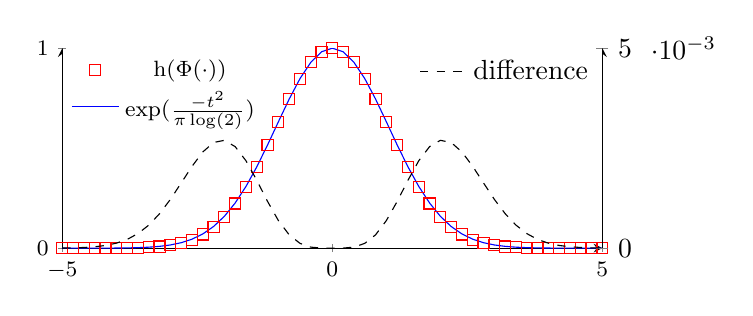
\begin{tikzpicture}

\begin{axis}[%
footnotesize,
scale only axis,
width=2.7in,
height=1.0in,
xmin=-5, xmax=5,
ymin=0, ymax=1,
xtick={-5,0,5},
ytick = {0,1},
axis y line = left,
axis x line = bottom,
legend style={ at={(0,1)}, anchor=north west, draw = none}]
]

\addplot [
color=red,
only marks,
mark=square,
mark options={solid}
]
coordinates{ (-5,6.64369e-06) (-4.8,1.72218e-05) (-4.6,4.2873e-05) (-4.4,0.000102503) (-4.2,0.000235365) (-4,0.000519064) (-3.8,0.0010995) (-3.6,0.00223711) (-3.4,0.00437257) (-3.2,0.00821083) (-3,0.0148147) (-2.8,0.0256873) (-2.6,0.0428103) (-2.4,0.0685917) (-2.2,0.105681) (-2,0.156615) (-1.8,0.223311) (-1.6,0.306444) (-1.4,0.40484) (-1.2,0.515021) (-1,0.631083) (-0.8,0.745014) (-0.6,0.847502) (-0.4,0.929133) (-0.2,0.981797) (0,1) (0.2,0.981797) (0.4,0.929133) (0.6,0.847502) (0.8,0.745014) (1,0.631083) (1.2,0.515021) (1.4,0.40484) (1.6,0.306444) (1.8,0.223311) (2,0.156615) (2.2,0.105681) (2.4,0.0685917) (2.6,0.0428103) (2.8,0.0256873) (3,0.0148147) (3.2,0.00821083) (3.4,0.00437257) (3.6,0.00223711) (3.8,0.0010995) (4,0.000519064) (4.2,0.000235365) (4.4,0.000102503) (4.6,4.2873e-05) (4.8,1.72218e-05) (5,6.64369e-06)
};
%\label{plots:approx_true}
\addlegendentry{$\mathrm{h}(\Phi(\cdot))$}

\addplot [
color=blue,
solid
]
coordinates{ (-5,1.03285e-05) (-4.8,2.54061e-05) (-4.6,6.02395e-05) (-4.4,0.00013768) (-4.2,0.000303323) (-4,0.000644146) (-3.8,0.00131859) (-3.6,0.00260182) (-3.4,0.0049487) (-3.2,0.00907298) (-3,0.0160344) (-2.8,0.0273151) (-2.6,0.0448534) (-2.4,0.0709961) (-2.2,0.108322) (-2,0.159311) (-1.8,0.22585) (-1.6,0.30863) (-1.4,0.406537) (-1.2,0.516189) (-1,0.631774) (-0.8,0.745348) (-0.6,0.847622) (-0.4,0.929159) (-0.2,0.981799) (0,1) (0.2,0.981799) (0.4,0.929159) (0.6,0.847622) (0.8,0.745348) (1,0.631774) (1.2,0.516189) (1.4,0.406537) (1.6,0.30863) (1.8,0.22585) (2,0.159311) (2.2,0.108322) (2.4,0.0709961) (2.6,0.0448534) (2.8,0.0273151) (3,0.0160344) (3.2,0.00907298) (3.4,0.0049487) (3.6,0.00260182) (3.8,0.00131859) (4,0.000644146) (4.2,0.000303323) (4.4,0.00013768) (4.6,6.02395e-05) (4.8,2.54061e-05) (5,1.03285e-05)
};
%\label{plots:approx_approx}
\addlegendentry{$\exp(\frac{-t^2}{\pi\log(2)})$}

\end{axis}

\begin{axis}[%
scale only axis,
width=2.7in,
height=1.0in,
xmin=-5, xmax=5,
ymin=0, ymax=0.005,
xtick={-5,0,5},
ytick = {0,0.005},
axis y line = right,
axis x line = none,
legend style={ at={(1,1)}, anchor=north east, draw = none}]
]

\addplot [
color=black,
dashed
]
coordinates{ (-5,3.68482e-06) (-4.8,8.18427e-06) (-4.6,1.73665e-05) (-4.4,3.51775e-05) (-4.2,6.79579e-05) (-4,0.000125081) (-3.8,0.000219088) (-3.6,0.000364708) (-3.4,0.000576126) (-3.2,0.000862153) (-3,0.00121977) (-2.8,0.00162773) (-2.6,0.00204316) (-2.4,0.00240434) (-2.2,0.0026417) (-2,0.00269602) (-1.8,0.00253851) (-1.6,0.00218519) (-1.4,0.00169772) (-1.2,0.00116807) (-1,0.000690885) (-0.8,0.000334143) (-0.6,0.000120243) (-0.4,2.60299e-05) (-0.2,1.71855e-06) (0,-0) (0.2,1.71855e-06) (0.4,2.60299e-05) (0.6,0.000120243) (0.8,0.000334143) (1,0.000690885) (1.2,0.00116807) (1.4,0.00169772) (1.6,0.00218519) (1.8,0.00253851) (2,0.00269602) (2.2,0.0026417) (2.4,0.00240434) (2.6,0.00204316) (2.8,0.00162773) (3,0.00121977) (3.2,0.000862153) (3.4,0.000576126) (3.6,0.000364708) (3.8,0.000219088) (4,0.000125081) (4.2,6.79579e-05) (4.4,3.51775e-05) (4.6,1.73665e-05) (4.8,8.18427e-06) (5,3.68482e-06)
};
%\label{plots:approx_error}
\addlegendentry{difference}

\end{axis}
\end{tikzpicture}

\caption{Analytic approximation to the binary entropy of the error function by a squared exponential.
The absolute error is always smaller than $3 \cdot 10^{-3}$. \label{fig:trick}}
\end{figure}

\section{Expectation propagation and variational Bayes\label{sec:EPinference}}

In this section, we describe in detail the proposed method for approximate inference in the multi-task preference learning model.
This method is based on the combination of expectation propagation \cite{Minka2002,gerven2010a}
and variational inference \cite{stern2009}. We first describe the general version of the method.
Finally, in Section \ref{sec:sparse}, we describe the version which employs sparse approximations to the covariance matrices $\mathbf{K}_\text{users}$
and $\mathbf{K}_\text{items}$ for speeding up computations.

The proposed EP method approximates the exact posterior distribution by the following parametric distribution:
\begin{eqnarray}
\mathcal{Q}(\mathbf{G}^{(\mathcal{D})},\mathbf{W},\mathbf{H}) & = & \left[\prod_{u=1}^{U}\prod_{d=1}^{D}\mathcal{N}(w_{ud}|m_{u,d}^{w},v_{u,d}^{w})\right]
\left[\prod_{d=1}^{D}\prod_{i=1}^{P} \mathcal{N}(h_{d,i}|m_{d,i}^h,v_{d,i}^{h})\right]\nonumber\\
& & \left[\prod_{u=1}^N \prod_{j=1}^{M_u} \mathcal{N}(g_{u,z_{u,j}}|m_{u,j}^g,v_{u,j}^g)\right]\,,\label{eq:epPostApprox}
\end{eqnarray}
where $m_{u,d}^w$, $v_{u,d}^w$, $m_{d,i}^h$, $v_{d,i}^h$,
$m_{u,j}^g$, and $v_{u,j}^g$ are free parameters to be determined by EP. 
The joint distribution of the model parameters and the data 
$\mathcal{P}(\mathbf{G}^{(\mathcal{D})},\mathbf{W},\mathbf{H},\mathbf{T}^{(\mathcal{D})},\mathbf{X},\ell)$ can be factorized
into four factors $f_1,\ldots,f_4$, namely,
\begin{equation}
\mathcal{P}(\mathbf{G}^{(\mathcal{D})},\mathbf{W},\mathbf{H},\mathbf{T}^{(\mathcal{D})},\mathbf{X},\ell) =
\prod_{k=1}^4 f_a(\mathbf{G}^{(\mathcal{D})},\mathbf{W},\mathbf{H})\,,
\end{equation}
where $f_1(\mathbf{G}^{(\mathcal{D})},\mathbf{W},\mathbf{H}) = \mathcal{P}(\mathbf{T}^{(\mathcal{D})}|\mathbf{G}^{(\mathcal{D})})$,
$f_2(\mathbf{G}^{(\mathcal{D})},\mathbf{W},\mathbf{H}) = \mathcal{P}(\mathbf{G}^{(\mathcal{D})}|\mathbf{W},\mathbf{H})$,
$f_3(\mathbf{G}^{(\mathcal{D})},\mathbf{W},\mathbf{H}) = \mathcal{P}(\mathbf{W}|\mathbf{U})$ and
$f_4(\mathbf{G}^{(\mathcal{D})},\mathbf{W},\mathbf{H}) = \mathcal{P}(\mathbf{H}|\mathbf{X},\ell)$.
EP approximates each of these exact factors by 
approximate factors $\hat{f}_{1}(\mathbf{W},\mathbf{H},\mathbf{G}^{(\mathcal{D})}),\ldots,\hat{f}_{4}(\mathbf{W},\mathbf{H},\mathbf{G}^{(\mathcal{D})})$
that have the same functional form as (\ref{eq:epPostApprox}), namely,
\begin{eqnarray}
\hat{f}_a(\mathbf{G}^{(\mathcal{D})},\mathbf{W},\mathbf{H}) & = &
\left[\prod_{u=1}^{U}\prod_{d=1}^{D}\mathcal{N}(w_{ud}|\hat{m}_{u,d}^{a,w},\hat{v}_{u,d}^{a,w})\right]
\left[\prod_{d=1}^{D}\prod_{i=1}^{P} \mathcal{N}(h_{d,i}|\hat{m}_{d,i}^{a,h},\hat{v}_{d,i}^{a,h})\right]\nonumber\\
& & \left[\prod_{u=1}^N \prod_{j=1}^{M_u} \mathcal{N}(g_{u,z_{u,j}}|\hat{m}_{u,j}^{a,g},\hat{v}_{u,j}^{a,g})\right] \hat{s}_a\,,
\end{eqnarray}
where $a=1,\ldots,4$ and $\hat{m}_{u,d}^{a,w}$, $\hat{v}_{u,d}^{a,w}$, $\hat{m}_{d,i}^{a,h}$, $\hat{v}_{d,i}^{a,h}$,
$\hat{m}_{u,j}^{a,g}$, $\hat{v}_{u,j}^{a,g}$ and $\hat{s}_a$ are free parameters to be determined by EP. 
The posterior approximation $\mathcal{Q}(\mathbf{w},\mathbf{H},\mathbf{G}^{(\mathcal{D})})$
is obtained as the normalized product of the approximate factors $\hat{f}_{1},\ldots,\hat{f}_{4}$, that is,
\begin{equation}
\mathcal{Q}(\mathbf{W},\mathbf{H},\mathbf{G}^{(\mathcal{D})}) \propto
\hat{f}_{1}(\mathbf{W},\mathbf{H},\mathbf{G}^{(\mathcal{D})})\cdots\hat{f}_{4}(\mathbf{W},\mathbf{H},\mathbf{G}^{(\mathcal{D})})\,.
\end{equation}
The first step of EP is to initialize all the approximate factors $\hat{f}_1,\ldots,\hat{f}_4$ and the posterior approximation $\mathcal{Q}$ to be uniform.
In particular,
$m_{u,d}^w=m_{d,i}^h=m_{u,j}^g=\hat{m}_{u,d}^{w,a}=\hat{m}_{d,i}^{a,h}=\hat{m}_{u,j}^{g,a}=0$ and 
$v_{u,d}^w = v_{d,i}^h = v_{u,j}^g = \hat{v}_{u,d}^{a,w} = \hat{v}_{d,i}^{a,h} = \hat{v}_{u,j}^{a,h} = \infty$ for
$a=1,\ldots,4$, $u=1,\ldots,U$, $d=1,\ldots,D$, $i=1,\ldots,P$ and $j = 1,\ldots,M_u$.
After that, EP refines the parameters of the approximate factors by iteratively minimizing the Kullback-Leibler (KL) divergence
between $\mathcal{Q}^{\setminus a}(\mathbf{W},\mathbf{H},\mathbf{G}^{(\mathcal{D})})f_a(\mathbf{W},\mathbf{H},\mathbf{G}^{(\mathcal{D})})$
and $\mathcal{Q}^{\setminus a}(\mathbf{W},\mathbf{H},\mathbf{G}^{(\mathcal{D})})\hat{f}_a(\mathbf{W},\mathbf{H},\mathbf{G}^{(\mathcal{D})})$, for $a=1,\ldots,4$,
where $\mathcal{Q}^{\setminus a}$ is the ratio between $\mathcal{Q}$ and $\hat{f}_a$. That is, EP iteratively minimizes
\begin{equation} 
\text{D}_{\text{KL}}(Q^{\setminus a}f_a\|Q^{\setminus a}\hat{f}_a) 
= \int \left[Q^{\setminus a}f_a \log \frac{Q^{\setminus a}f_a}{Q^{\setminus a}\hat{f}_a}+
Q^{\setminus a}\hat{f}_a-Q^{\setminus a}f_a\right]\,d\mathbf{W}\,d\mathbf{H}\,d\mathbf{G}^{(\mathcal{D})}\label{eq:KL}
\end{equation}
with respect to $\hat{f}_a$, for $a = 1,\ldots,4$.
The arguments to $Q^{\setminus a}f_a $ and 
$Q^{\setminus a}\hat{f}_a$ have been omitted in the 
right-hand side of (\ref{eq:KL}) to improve the readability of the expression.
However, the minimization of (\ref{eq:KL}) does not perform well when we have to refine the parameters of $\hat{f}_2$.
The reason for this is that the corresponding exact factor $f_2$ (equation (7) in the main document)
is invariant to simultaneous changes in sign, scalings, or rotations of the entries of $\mathbf{W}$ and $\mathbf{H}$.
This non-identifiability in the latent space spanned by $\mathbf{W}$ and $\mathbf{H}$
originates multiple modes in the distribution $Q^{\setminus 2}f_2$.
The minimization of the direct version of the KL divergence results in an approximation that averages across all
of the modes, leading to poor predictive performance.
We solve this problem by following an approach similar to the one described by \cite{stern2009}.
Instead of minimizing $\text{KL}(\mathcal{Q}^{\setminus 2} f_2 \| \mathcal{Q}^{\setminus 2} \hat{f}_2)$,
we refine $\hat{f}_2$ by minimizing the reversed version of the KL divergence, that is,
we minimize $\text{KL}(\mathcal{Q}^{\setminus 2} \hat{f}_2 \| \mathcal{Q}^{\setminus 2} f_2)$ with respect to the parameters of $\hat{f}_2$.
The reversed version of the divergence has mode seeking properties \citep{Bishop2007} and tends to approximate
only a single mode of the target distribution, leading to better predictive accuracy.

The EP algorithm iteratively refines the approximate factors until convergence.
We assume the algorithm has converged when the absolute value of the change in the parameters
$m_{u,i}^g$ of $\mathcal{Q}$, where $u = 1,\ldots,U$ and $i = 1,\ldots,M_u$,
is less than a threshold $\delta = 10^{-2}$ between two consecutive cycles of EP,
where a cycle consists in the sequential update of all the approximate factors.
However, convergence is not guaranteed and
EP may end up oscillating without ever stopping \citep{Minka2001}.
This undesirable behavior can be prevented by \emph{damping} the EP updates \citep{Minka2002}.
Let $\hat{f}_a^\text{new}$ denote the value of the approximate factor that minimizes the Kullback-Leibler
divergence. Damping consists in using
\begin{equation}
\hat{f}_a^\text{damp} = \left[ \hat{f}_a^\text{new} \right]^\epsilon \left[ \hat{f}_a \right]^{(1 - \epsilon)}\,,\label{eq:damping}
\end{equation}
instead of $\hat{f}_a^\text{new}$ for the update of each approximate factor $a = 1,\ldots,4$.
The quantity $\hat{f}_a$ represents in (\ref{eq:damping})
the factor before the update. The parameter
$\epsilon \in [0,1]$ controls the amount of damping.
The original EP update (that is, without damping)
is recovered in the limit $\epsilon = 1$. For $\epsilon = 0$,
the approximate factor $\hat{f}_a$ is not modified.
To improve the converge of EP, we use a damping scheme
with a parameter $\epsilon$ that is initialized to 1
and then progressively annealed as recommended by \cite{HernandezLobato2010}.
After each iteration of EP, the value of
this parameter is multiplied by a constant $k < 1$.
The value selected for $k$ is $k = 0.95$.
In the experiments performed, EP performs on average about 50 iterations.

\subsection{The EP predictive distribution}

EP can also approximate the predictive distribution, given by equation (11) in the main manuscript. 
For this, we replace the exact posterior with the EP approximation $\mathcal{Q}$. In this way, we obtain
\begin{equation}
\mathcal{P}(t_{u,P+1}|\mathbf{T}^{(\mathcal{D})},\mathbf{X},\ell,p_{P+1}) \approx 
\Phi\left[t_{u,P+1} m_{u,P+1}^g(v_{u,P+1}^g + 1)^{-\frac{1}{2}}\right]\,,
\end{equation}
where
\begin{align}
m_{u,P+1}^g & = \sum_{d=1}^D  m_{u,d}^w m_{d,P+1}^h\,,\\
v_{u,P+1}^g & = \sum_{d=1}^D  [m_{u,d}^w]^2 v_{d,P+1}^h + \sum_{d=1}^D v_{u,d}^w [m_{d,P+1}^h]^2 + \sum_{d=1}^D v_{u,d}^w v_{d,P+1}^h
\end{align}
and $m_{d,P+1}^h$ and $v_{d,P+1}^h$ for $d = 1,\ldots,D$ are given by
\begin{align}
m_{d,P+1}^h & = \mathbf{k}_\star^\text{T} \left[ \mathbf{K}_\text{items} +
\text{diag}[\hat{\mathbf{v}}_d^{h,2}] \right]^{-1} \hat{\mathbf{m}}_d^{h,2}\,,\label{eq:predictiveMean}\\
v_{d,P+1}^h & = k_\star - \mathbf{k}_\star^\text{T} \left[ \mathbf{K}_\text{items} +
\text{diag}[\hat{\mathbf{v}}_d^{h,2}] \right]^{-1} \mathbf{k}_\star\,,\label{eq:predictiveVariance}
\end{align}
where $k_\star$ is the prior variance of $h_d(\mathbf{x}_{\alpha(P+1)}, \mathbf{x}_{\beta(P+1)})$,
$\mathbf{k}_\star$ is a $P$-dimensional vector that contains the prior covariances between $h_d(\mathbf{x}_{\alpha(P+1)}, \mathbf{x}_{\beta(P+1)})$
and $h_d(\mathbf{x}_{\alpha(1)}, \mathbf{x}_{\beta(1)}),\ldots,h_d(\mathbf{x}_{\alpha(P)}, \mathbf{x}_{\beta(P)})$ for $d=1,\ldots,D$,
the function $\text{diag}(\cdot)$ applied to a vector returns a diagonal matrix with that vector in
its diagonal and the vectors $\hat{\mathbf{m}}_d^{h,2}$ and $\hat{\mathbf{v}}_d^{h,2}$ are given by
$\hat{\mathbf{m}}_d^{h,2}=(\hat{m}_{1,d}^{h,2},\ldots,\hat{m}_{P,d}^{h,2})^\text{T}$ and
$\hat{\mathbf{v}}_d^{h,2}=(\hat{v}_{1,d}^{h,2},\ldots,\hat{v}_{P,d}^{h,2})^\text{T}$.

\subsection{The EP update operations}

In this section we describe the EP updates for refining the approximate factors $\hat{f}_1,\ldots,\hat{f}_4$.
For the sake of clarity, we only include the update rules with no damping ($\epsilon = 1$).
Incorporating the effect of damping in these operations is straightforward. 
With damping,  the natural parameters of the approximate factors become 
a convex combination of the natural parameters before and after the 
update with no damping
\begin{align}
[\hat{v}_{u,d}^{w,a}]^{-1}_\text{damp} & = \epsilon [\hat{v}_{u,d}^{w,a}]^{-1}_\text{new}
+ (1 - \epsilon) [\hat{v}_{u,d}^{w,a}]^{-1}_\text{old}\,,\\
[\hat{m}_{u,d}^{w,a}]_\text{damp} [\hat{v}_{u,d}^{w,a}]_\text{damp}^{-1} & =
\epsilon [\hat{m}_{u,d}^{w,a}]_\text{new} [\hat{v}_{u,d}^{w,a}]_\text{new}^{-1} + (1 - \epsilon)
[\hat{m}_{u,d}^{w,a}]_\text{old}[\hat{v}_{u,d}^{w,a}]^{-1}_\text{old}\,,\\
[\hat{v}_{d,i}^{h,a}]^{-1}_\text{damp} & = \epsilon [\hat{v}_{d,i}^{h,a}]^{-1}_\text{new}
+ (1 - \epsilon) [\hat{v}_{d,i}^{h,a}]^{-1}_\text{old}\,,\\
[\hat{m}_{d,i}^{h,a}]_\text{damp} [\hat{v}_{d,i}^{h,a}]_\text{damp}^{-1} & =
\epsilon [\hat{m}_{d,i}^{h,a}]_\text{new} [\hat{v}_{d,i}^{h,a}]_\text{new}^{-1} + (1 - \epsilon)
[\hat{m}_{d,i}^{h,a}]_\text{old}[\hat{v}_{d,i}^{h,a}]^{-1}_\text{old}\,,\\
[\hat{v}_{u,j}^{g,a}]^{-1}_\text{damp} & = \epsilon [\hat{v}_{u,j}^{g,a}]^{-1}_\text{new}
+ (1 - \epsilon) [\hat{v}_{u,j}^{g,a}]^{-1}_\text{old}\,,\\
[\hat{m}_{d,j}^{g,a}]_\text{damp} [\hat{v}_{u,j}^{g,a}]_\text{damp}^{-1} & =
\epsilon [\hat{m}_{u,j}^{g,a}]_\text{new} [\hat{v}_{u,j}^{g,a}]_\text{new}^{-1} + (1 - \epsilon)
[\hat{m}_{u,j}^{g,a}]_\text{old}[\hat{v}_{u,j}^{g,a}]^{-1}_\text{old}\,,
\end{align}
where $u = 1,\ldots,U$, $d = 1,\ldots,D$, $i = 1,\ldots,P$ and $j=1,\ldots,M_u$.
The subscript $\emph{new}$ denotes the value of the parameter 
given by the full EP update operation with no damping.
The subscript $\emph{damp}$ denotes the parameter value given by the
damped update rule. The subscript $\emph{old}$ refers to
the value of the parameter before the EP update.
The updates for the parameters $\hat{s}_1,\ldots,\hat{s}_4$ are not damped. These parameters are initialized to 1 and are only
updated once the EP algorithm has converged.

The first factor to be refined is $\hat{f}_4$. The update operations that minimize
$\text{KL}(\mathcal{Q}^{\setminus 4} f_4 \| \mathcal{Q}^{\setminus 4} \hat{f}_4)$ are given by
\begin{align}
[\hat{v}_{d,i}^{h,4}]_\text{new} & =
\left\{ [v_{d,i}^{h}]_\text{new}^{-1} - [\hat{v}_{d,i}^{h,2} ]_\text{old}^{-1}\right\}^{-1}\,,\\
[\hat{m}_{d,i}^{h,4}]_\text{new} & =
[\hat{v}_{d,i}^{h,4}]_\text{new} \left\{[ m_{d,i}^{h}]_\text{new} 
[v_{d,i}^{h}]_\text{new}^{-1} - [\hat{m}_{d,i}^{h,4}]_\text{old} [\hat{v}_{d,i}^{h,4}]_\text{old}^{-1}\right\}^{-1}\,,
\end{align}
for $d = 1,\ldots,D$ and $i = 1,\ldots,P$,
where the subscripts \emph{new} and \emph{old} denote the parameter value after and before the update, respectively, and
the parameters $[v_{d,i}^{h}]_\text{new}$ and $[ m_{d,i}^{h}]_\text{new}$ are the $i$-th entries in the vectors
$[\mathbf{v}_{d}^{h}]_\text{new}$ and $[\mathbf{m}_{d}^{h}]_\text{new}$ given by
\begin{align}
[\mathbf{v}_{d}^{h}]_\text{new} & = \text{diag}\left[ \bm \Sigma_d^h \right]\,,\label{eq:Sigmah} \\
[\mathbf{m}_{d}^{h}]_\text{new} & = \bm \Sigma_d^h \text{diag}[\hat{\mathbf{v}}_d^{h,2}]^{-1} \hat{\mathbf{m}}_d^{h,2}\label{eq:Sigma2h}\,,
\end{align}
where $[\bm \Sigma_d^h]^{-1} = \mathbf{K}^{-1}_\text{items} + \text{diag}[\hat{\mathbf{v}}_d^{h,2}]^{-1}$
and the vectors
$\hat{\mathbf{m}}_d^{h,2}$ and $\hat{\mathbf{v}}_d^{h,2}$ are $P$-dimensional vectors given by
$\hat{\mathbf{m}}_d^{h,2}=(\hat{m}_{1,d}^{h,2},\ldots,\hat{m}_{P,d}^{h,2})^\text{T}$ and
$\hat{\mathbf{v}}_d^{h,2}=(\hat{v}_{1,d}^{h,2},\ldots,\hat{v}_{P,d}^{h,2})^\text{T}$.

The second factor to be refined by EP is $\hat{f}_3$. The update operations that minimize
$\text{KL}(\mathcal{Q}^{\setminus 3} f_3 \| \mathcal{Q}^{\setminus 3} \hat{f}_3)$ are
\begin{align}
[\hat{v}_{u,d}^{w,3}]_\text{new} & =
\left\{ [v_{u,d}^{w}]_\text{new}^{-1} - [\hat{v}_{u,d}^{w,2} ]_\text{old}^{-1}\right\}^{-1}\,,\\
[\hat{m}_{u,d}^{w,3}]_\text{new} & =
[\hat{v}_{u,d}^{w,3}]_\text{new} \left\{[ m_{u,d}^{w}]_\text{new} 
[v_{u,d}^{w}]_\text{new}^{-1} - [\hat{m}_{u,d}^{w,3}]_\text{old} [\hat{v}_{u,d}^{w,3}]_\text{old}^{-1}\right\}^{-1}\,,
\end{align}
for $u = 1,\ldots,U$ and $d = 1,\ldots,D$,
where the parameters $[v_{u,d}^{w}]_\text{new}$ and $[ m_{u,d}^{w}]_\text{new}$ are the $u$-th entries in the vectors
$[\mathbf{v}_{d}^{w}]_\text{new}$ and $[\mathbf{m}_{d}^{w}]_\text{new}$ given by
\begin{align}
[\mathbf{v}_{d}^{w}]_\text{new} & = \text{diag}\left[ \bm \Sigma_d^w \right]\,,\label{eq:Sigmaw} \\
[\mathbf{m}_{d}^{w}]_\text{new} & = \bm \Sigma_d^w \text{diag}[\hat{\mathbf{v}}_d^{w,2}]^{-1} \hat{\mathbf{m}}_d^{w,2}\label{eq:Sigma2w}\,,
\end{align}
where $[ \bm \Sigma_d^w]^{-1} = \mathbf{K}^{-1}_\text{items} + \text{diag}[\hat{\mathbf{v}}_d^{w,2}]^{-1}$ and
the vectors $\hat{\mathbf{m}}_d^{w,2}$ and $\hat{\mathbf{v}}_d^{w,2}$ are given by
$\hat{\mathbf{m}}_d^{w,2}=(\hat{m}_{1,d}^{w,2},\ldots,\hat{m}_{U,d}^{w,2})^\text{T}$ and
$\hat{\mathbf{v}}_d^{w,2}=(\hat{v}_{1,d}^{w,2},\ldots,\hat{v}_{U,d}^{w,2})^\text{T}$.

The third factor to be refined by EP is $\hat{f}_2$. For this, we follow the approach used by \cite{stern2009}
and first marginalize $f_2\mathcal{Q}^{\setminus 2}$ with respect to $\mathbf{G}^{(\mathcal{D})}$.
The result of this operation is the auxiliary un-normalized distribution $\mathcal{S}(\mathbf{W},\mathbf{H})$ given by
\begin{eqnarray}
\mathcal{S}(\mathbf{W},\mathbf{H}) & = & \int 
\prod_{u=1}^{U} \prod_{i=1}^{M_u}\delta[g_{u,z_{u,i}}-\mathbf{w}_u\mathbf{h}_{\cdot,z_{u,i}}]
\mathcal{Q}^{\setminus 2 }(\mathbf{G}^{(\mathcal{D})},\mathbf{W},\mathbf{H})\,d\mathbf{G}^{(\mathcal{D})}\nonumber\\
& = & \left[\prod_{u=1}^{U}
\prod_{i=1}^{M_u}\mathcal{N}(\mathbf{w}_u\mathbf{h}_{\cdot,z_{u,i}}|\hat{m}^{g,1}_{u,i},\hat{v}^{g,1}_{u,i})\right]
\left[ \prod_{u=1}^U\prod_{d=1}^D \mathcal{N}(w_{u,d}|\hat{m}^{w,3}_{u,d},\hat{v}^{w,3}_{u,d}) \right]\nonumber \\
& & \left[ \prod_{d=1}^D\prod_{i=1}^P \mathcal{N}(h_{d,i}|\hat{m}^{h,4}_{d,i},\hat{v}^{h,4}_{d,i}) \right]\,.
\end{eqnarray}
Let $\mathcal{Q}_{\mathbf{W},\mathbf{H}}$ be the posterior approximation (\ref{eq:epPostApprox}) after marginalizing $\mathbf{G}^{(\mathcal{D})}$ out.
The parameters of $\mathcal{Q}_{\mathbf{W},\mathbf{H}}$, that is, $m_{d,i}^{h}$,
$v_{d,i}^{h}$, $m_{u,d}^{w}$ and $v_{u,d}^{w}$, for $d = 1,\ldots,D$, $u=1,\ldots,U$ and $i = 1,\ldots,P$,
are then optimized to minimize $\text{KL}(\mathcal{Q}_{\mathbf{W},\mathbf{H}}\|\mathcal{S})$.
This can be done very efficiently using the gradient descent method described by \cite{raiko2007}. The resulting EP updates for $\hat{f}_2$ are
given by
\begin{align}
[\hat{v}_{d,i}^{h,2}]_\text{new} & =
\left\{ [v_{d,i}^{h}]_\text{new}^{-1} - [\hat{v}_{d,i}^{h,2} ]_\text{old}^{-1}\right\}^{-1}\,,\\
[\hat{m}_{d,i}^{h,2}]_\text{new} & =
[\hat{v}_{d,i}^{h,2}]_\text{new} \left\{[ m_{d,i}^{h}]_\text{new} 
[v_{d,i}^{h}]_\text{new}^{-1} - [\hat{m}_{d,i}^{h,2}]_\text{old} [\hat{v}_{d,i}^{h,2}]_\text{old}^{-1}\right\}^{-1}\,,\\
[\hat{v}_{u,d}^{w,2}]_\text{new} & =
\left\{ [v_{u,d}^{w}]_\text{new}^{-1} - [\hat{v}_{u,l}^{w,2} ]_\text{old}^{-1}\right\}^{-1}\,,\\
[\hat{m}_{u,d}^{w,2}]_\text{new} & =
[\hat{v}_{u,d}^{w,2}]_\text{new} \left\{[ m_{u,d}^{w}]_\text{new} 
[v_{u,d}^{w}]_\text{new}^{-1} - [\hat{m}_{u,d}^{w,2}]_\text{old} [\hat{v}_{u,d}^{w,2}]_\text{old}^{-1}\right\}^{-1}\,,\\
[\hat{v}_{u,j}^{g,2}]_\text{new} & =
\left\{ [v_{u,j}^{g}]_\text{new}^{-1} - [\hat{v}_{u,j}^{g,2} ]_\text{old}^{-1}\right\}^{-1}\,,\\
[\hat{m}_{u,j}^{g,2}]_\text{new} & =
[\hat{v}_{u,j}^{g,2}]_\text{new} \left\{[ m_{u,j}^{g}]_\text{new} 
[v_{u,j}^{g}]_\text{new}^{-1} - [\hat{m}_{u,j}^{g,2}]_\text{old} [\hat{v}_{u,j}^{g,2}]_\text{old}^{-1}\right\}^{-1}\,,
\end{align}
for $d = 1,\ldots,D$, $u = 1,\ldots,U$, $j = 1,\ldots,M_u$ and $i = 1,\ldots,P$ where $[m_{d,i}^{h}]_\text{new}$,
$[v_{d,i}^{h}]_\text{new}$, $[ m_{u,d}^{w}]_\text{new}$ and $[v_{u,d}^{w}]_\text{new}$, are the parameters of $\mathcal{Q}$ that minimize
$\text{KL}(\mathcal{Q}_{\mathbf{W},\mathbf{H}}\|\mathcal{S})$ and
\begin{align}
[m_{u,j}^{g}]_\text{new} & = \sum_{d=1}^D [m_{u,d}^{w}]_\text{new} [m_{d,z_{u,j}}^{h}]_\text{new}\,,\\
[v_{u,j}^{g}]_\text{new} & = \sum_{d=1}^D [m_{u,d}^{w}]_\text{new}^2 [v_{d,z_{u,j}}^{h}]_\text{new} +
\sum_{d=1}^D [v_{u,d}^{w}]_\text{new} [m_{d,z_{u,j}}^{h}]_\text{new}^2 +
\sum_{d=1}^D [v_{u,d}^{w}]_\text{new} [v_{d,z_{u,j}}^{h}]_\text{new}\,.
\end{align}

The last factor to be refined on each cycle of EP is $\hat{f}_1$. The EP update operations for this factor are
\begin{align}
[\hat{m}_{u,i}^{g,1}]_\text{new} & = \hat{m}_{u,i}^{g,2} + \hat{v}_{u,i}^{g,2}
[m_{u,i}]^{-1}_\text{new}\,,\\
[\hat{v}_{u,i}^{g,1}]_\text{new} & = \hat{v}_{u,i}^{g,2} \left[ \alpha_{u,i}^{-1} [m_{u,i}]^{-1}_\text{new} - 1 \right]\,,
\end{align}
for $u = 1,\ldots,U$ and $i = 1,\ldots,M_u$, where
\begin{align}
[m_{u,i}]_\text{new} & = \hat{m}_{u,i}^{g,2} + \hat{v}_{u,i}^{g,2} \alpha_{u,i}\,,\\
\alpha_{u,i} & = \Phi[\beta_{u,i}]^{-1} \phi[\beta_{u,i}] t_{u,i} [\hat{v}_{u,i}^{g,2} + 1]^{-\frac{1}{2}}\,,\\
\beta_{u,i} & = t_{u,i} \hat{m}_{u,i}^{g,2} [\hat{v}_{u,i}^{g,2} + 1]^{-\frac{1}{2}}
\end{align}
and $\phi$ and $\Phi$ are the density and the cumulative probability functions of a standard Gaussian distribution,
respectively.

\subsection{The EP approximation of the model evidence}

Once EP has converged, we can approximate the evidence of the model, that is, $\mathcal{P}(\mathbf{T}^{(\mathcal{D})}|\mathbf{X},\ell)$, using
\begin{align}
\mathcal{P}(\mathbf{T}^{(\mathcal{D})}|\mathbf{X},\ell) \approx \int \prod_{a=1}^4
\hat{f}_a(\mathbf{G}^{(\mathcal{D})},\mathbf{W},\mathbf{H})\,d\mathbf{G}^{(\mathcal{D})}\,d\mathbf{H}\,d\mathbf{W}\,.
\end{align}
For this, we have to compute the value of the parameters $\hat{s}_1,\ldots,\hat{s}_4$. The value of $\hat{s}_1$ is
\begin{equation}
\log\hat{s}_1 = \sum_{u=1}^{U}\sum_{i=1}^{M_u}\left[\log \Phi[\beta_{u,i}] +
\frac{1}{2}\log(2\pi)+\frac{1}{2}\log \frac{\hat{v}_{u,i}^{g,1} \hat{v}_{u,i}^{g,2}}{v_{u,i}^g}-
\frac{[m_{u,i}^g]^2}{2v_{u,i}^g}+\frac{[\hat{m}_{u,i}^{g,1}]^2}{2\hat{v}_{u,i}^{g,1}}+
\frac{[\hat{m}_{u,i}^{g,2}]^2}{2\hat{v}_{u,i}^{g,2}}\right]\,.
\end{equation}
The value of $\hat{s}_2$ is given by
\begin{align}
\log\hat{s}_2 & = \log Z_2 + \sum_{u=1}^{U}\sum_{i=1}^{M_u}\left[\frac{1}{2}\log(2\pi)+
\frac{1}{2}\log \frac{\hat{v}_{u,i}^{g,1}\hat{v}_{u,i}^{g,2}}{v_{u,i}^g}-
\frac{[m_{u,i}^g]^2}{2v_{u,i}^g}+\frac{[\hat{m}_{u,i}^{g,1}]^2}{2\hat{v}_{u,i}^{g,1}}+
\frac{[\hat{m}_{u,i}^{g,2}]^2}{2\hat{v}_{u,i}^{g,2}}\right]+\nonumber\\
& \quad \sum_{d=1}^{D}\sum_{i=1}^{P}\left[\frac{1}{2}\log(2\pi)+
\frac{1}{2}\log \frac{\hat{v}_{d,i}^{h,2}\hat{v}_{d,i}^{h,4}}{v_{d,i}^h}-
\frac{[m_{d,i}^h]^2}{2v_{d,i}^h}+\frac{[\hat{m}_{d,i}^{h,2}]^2}{2\hat{v}_{d,i}^{h,2}}+
\frac{[\hat{m}_{d,i}^{h,4}]^2}{2\hat{v}_{d,i}^{h,4}}\right]+\nonumber\\
& \quad \sum_{u=1}^{U}\sum_{d=1}^{D}\left[\frac{1}{2}\log(2\pi)+
\frac{1}{2}\log \frac{\hat{v}_{u,d}^{w,2}\hat{v}_{u,d}^{w,3}}{v_{u,d}^w}-
\frac{[m_{u,d}^w]^2}{2v_{u,d}^w}+\frac{[\hat{m}_{u,d}^{w,2}]^2}{2\hat{v}_{u,d}^{w,2}}+
\frac{[\hat{m}_{u,d}^{w,3}]^2}{2\hat{v}_{u,d}^{w,3}}\right]\,,
\end{align}
where $Z_2$ is the variational lower bound obtained in the update of $\hat{f}_2$, that is,
\begin{equation}
Z_2 = \int \mathcal{Q}_{\mathbf{W},\mathbf{H}}\log\frac{\mathcal{S}(\mathbf{W},\mathbf{H})}
{\mathcal{Q}_{\mathbf{W},\mathbf{H}}(\mathbf{W},\mathbf{H})} \,d\mathbf{W},d\mathbf{H}\,.
\end{equation}
The value of $\tilde{s}_{3}$ is given by
\begin{align}
\log\hat{s}_3 = \log Z_3 + \sum_{d=1}^{D}\sum_{u=1}^{U}\left[
\frac{1}{2}\log(2\pi)+\frac{1}{2}\log \frac{\hat{v}_{u,d}^{w,3} \hat{v}_{u,d}^{w,2}}{v_{u,d}^w}-
\frac{[m_{u,d}^w]^2}{2v_{u,d}^w}+\frac{[\hat{m}_{u,d}^{w,3}]^2}{2\hat{v}_{u,d}^{w,3}}+
\frac{[\hat{m}_{u,d}^{w,2}]^2}{2\hat{v}_{u,d}^{w,2}}\right]\,,
\end{align}
where $Z_3$ is computed using
\begin{eqnarray}
\log Z_{3} & = & \log \int \mathcal{P}(\mathbf{W}|\mathbf{U})\left[\prod_{u=1}^{U}\prod_{d=1}^{D}
\mathcal{N}(w_{u,d}|\hat{m}_{u,d}^{w,2},\hat{m}_{u,d}^{w,2})\right]d\mathbf{W}\nonumber\\
& = & -\frac{DP}{2}\log(2\pi) + \frac{1}{2}\sum_{d=1}^D\log|\bm \Sigma_d^w| -
\frac{D}{2}\log|\mathbf{K}_\text{users}| - \frac{1}{2} \sum_{u=1}^U\sum_{d=1}^D \log \hat{v}_{u,d}^{w,2} - \nonumber \\
& & \frac{1}{2} \sum_{u=1}^U\sum_{d=1}^D \frac{[\hat{m}_{u,d}^{w,2}]^2}{\hat{v}_{u,d}^{w,2}} +
\frac{1}{2} \sum_{d=1}^D [\mathbf{m}_d^w]^\text{T} \bm [\Sigma_d^w]^{-1} \mathbf{m}_d^w\,,\label{eq:Z3}
\end{eqnarray}
and $[ \bm \Sigma_d^w]^{-1} = \mathbf{K}^{-1}_\text{users} + \text{diag}[\hat{\mathbf{v}}_d^{w,2}]^{-1}$,
$\mathbf{m}_d^w = \bm \Sigma_d^w \text{diag}[\hat{\mathbf{v}}_d^{w,2}]^{-1} \hat{\mathbf{m}}_d^{w,2}$
and the vectors $\hat{\mathbf{m}}_d^{w,2}$ and $\hat{\mathbf{v}}_d^{w,2}$ are given by
$\hat{\mathbf{m}}_d^{w,2}=(\hat{m}_{1,d}^{w,2},\ldots,\hat{m}_{U,d}^{w,2})^\text{T}$ and
$\hat{\mathbf{v}}_d^{w,2}=(\hat{v}_{1,d}^{w,2},\ldots,\hat{v}_{U,d}^{w,2})^\text{T}$.
Finally, the value of $\tilde{s}_{4}$ is given by
\begin{align}
\log\hat{s}_4 = \log Z_4 + \sum_{d=1}^{D}\sum_{i=1}^{P}\left[
\frac{1}{2}\log(2\pi)+\frac{1}{2}\log \frac{\hat{v}_{d,i}^{h,4} \hat{v}_{d,i}^{h,2}}{v_{d,i}^h}-
\frac{[m_{d,i}^h]^2}{2v_{d,i}^h}+\frac{[\hat{m}_{d,i}^{h,4}]^2}{2\hat{v}_{d,i}^{h,4}}+
\frac{[\hat{m}_{d,i}^{h,2}]^2}{2\hat{v}_{d,i}^{h,2}}\right]\,,
\end{align}
where $Z_4$ is computed using
\begin{eqnarray}
\log Z_{4}  & = & \log \int \mathcal{P}(\mathbf{H}|\mathbf{X},\ell)\left[\prod_{d=1}^{D}\prod_{i=1}^{P}
\mathcal{N}(h_{d,i}|\hat{m}_{d,i}^{h,2},\hat{m}_{d,i}^{h,2})\right]d\mathbf{H}\nonumber\\
& = & -\frac{DP}{2}\log(2\pi) + \frac{1}{2}\sum_{d=1}^D\log|\bm \Sigma_d^h| -
\frac{D}{2}\log|\mathbf{K}_\text{items}| - \frac{1}{2} \sum_{d=1}^D\sum_{i=1}^P \log \hat{v}_{d,i}^{h,2} - \nonumber \\
& & \frac{1}{2} \sum_{d=1}^D\sum_{i=1}^p \frac{[\hat{m}_{d,i}^{h,2}]^2}{\hat{v}_{d,i}^{h,2}} +
\frac{1}{2} \sum_{d=1}^D [\mathbf{m}_d^h]^\text{T} [\bm \Sigma_d^h]^{-1} \mathbf{m}_d^h\,,\label{eq:Z4}
\end{eqnarray}
and $[\bm \Sigma_d^h]^{-1} = \mathbf{K}^{-1}_\text{items} + \text{diag}[\hat{\mathbf{v}}_d^{h,2}]^{-1}$,
$\mathbf{m}_d^h = \bm \Sigma_d \text{diag}[\hat{\mathbf{v}}_d^{h,2}]^{-1} \hat{\mathbf{m}}_d^{h,2}$
and the vectors $\hat{\mathbf{m}}_d^{h,2}$ and $\hat{\mathbf{v}}_d^{h,2}$ are given by
$\hat{\mathbf{m}}_d^{h,2}=(\hat{m}_{1,d}^{h,2},\ldots,\hat{m}_{P,d}^{h,2})^\text{T}$ and
$\hat{\mathbf{v}}_d^{h,2}=(\hat{v}_{1,d}^{h,2},\ldots,\hat{v}_{P,d}^{h,2})^\text{T}$.
Given $\hat{s}_1,\ldots,\hat{s}_4$, we approximate $\mathcal{P}(\mathbf{T}^{(\mathcal{D})}|\mathbf{X},\ell)$ using
\begin{eqnarray}
\log \mathcal{P}(\mathbf{T}^{(\mathcal{D})}|\mathbf{X},\ell) & \approx & \sum_{i=a}^{4}\log\hat{s}_{a}-
\sum_{u=1}^{U}\sum_{i=1}^{M_u}\left[\frac{1}{2}\log(2\pi)+\frac{1}{2}\log \frac{\hat{v}_{u,i}^{g,1} \hat{v}_{u,i}^{g,2}}{v_{u,i}^g}-
\frac{[m_{u,i}^g]^2}{2v_{u,i}^g}+\frac{[\hat{m}_{u,i}^{g,1}]^2}{2\hat{v}_{u,i}^{g,1}}+
\frac{[\hat{m}_{u,i}^{g,2}]^2}{2\hat{v}_{u,i}^{g,2}}\right]-\nonumber\\
& & \sum_{d=1}^{D}\sum_{i=1}^{P}\left[
\frac{1}{2}\log(2\pi)+\frac{1}{2}\log \frac{\hat{v}_{d,i}^{h,4} \hat{v}_{d,i}^{h,2}}{v_{d,i}^h}-
\frac{[m_{d,i}^h]^2}{2v_{d,i}^h}+\frac{[\hat{m}_{d,i}^{h,4}]^2}{2\hat{v}_{d,i}^{h,4}}+
\frac{[\hat{m}_{d,i}^{h,2}]^2}{2\hat{v}_{d,i}^{h,2}}\right]-\nonumber\\
& & \sum_{u=1}^{U}\sum_{d=1}^{D}\left[\frac{1}{2}\log(2\pi)+
\frac{1}{2}\log \frac{\hat{v}_{u,d}^{w,2}\hat{v}_{u,d}^{w,3}}{v_{u,d}^w}-
\frac{[m_{u,d}^w]^2}{2v_{u,d}^w}+\frac{[\hat{m}_{u,d}^{w,2}]^2}{2\hat{v}_{u,d}^{w,2}}+
\frac{[\hat{m}_{u,d}^{w,3}]^2}{2\hat{v}_{u,d}^{2,3}}\right]\,.\label{eq:EPevidenceApprox}
\end{eqnarray}
Finally, some of the EP updates may generate a negative value for $\hat{v}_{u,i}^{g,a}$, 
$\hat{v}_{u,d}^{w,a}$ or $\hat{v}_{d,j}^{h,a}$, where $u = 1,\ldots,U$, $i = 1,\ldots,M_u$, $j = 1,\ldots,P$ and $i = 1,\ldots,4$.
Negative variances in Gaussian approximate factors 
are common in many EP implementations \citep{Minka2001,Minka2002}.
When this happens, the marginals of the approximate factor with negative 
variances are not density functions. Instead, they
are correction factors that compensate the errors in the corresponding marginals of other approximate factors.
However, these negative variances can lead to failure of the proposed EP algorithm.
This may happen when we have to compute $\log|\bm \Sigma_d^h|$ in (\ref{eq:Z4}) and some
of the $\hat{v}_{d,i}^{h,2}$ are negative. In this case, $\Sigma_d^h$ may not be
positive definite and $|\bm \Sigma_d^h|$ may be negative. The result is that EP may no longer be able to approximate the model evidence
since $\log |\bm \Sigma_d^h|$ may not be defined in (\ref{eq:Z4}).
The same may occur for $\log|\bm \Sigma_d^w|$ in (\ref{eq:Z3}).
To address this problem, whenever an EP update yields a negative number for any of the
$\hat{v}_{u,i}^{g,a}$, $\hat{v}_{u,d}^{w,a}$ or $\hat{v}_{d,j}^{h,a}$, we do not update this parameter, nor the corresponding
$\hat{m}_{u,i}^{g,a}$, $\hat{m}_{u,d}^{w,a}$ or $\hat{m}_{d,j}^{h,a}$.

\subsection{Sparse approximations to speed up computations} \label{sec:sparse}

The computational cost of EP is determined by the operations needed to refine the approximate factors $\hat{f}_3$ and $\hat{f}_4$.
In particular, computing the vectors $[\mathbf{v}_{d}^{h}]_\text{new}$ and $[\mathbf{m}_{d}^{h}]_\text{new}$ in
(\ref{eq:Sigmah}) and (\ref{eq:Sigma2h}), for $d = 1,\ldots,D$, has cost $\mathcal{O}(DP^3)$. Similarly,
the computation of the vectors $[\mathbf{v}_{d}^{w}]_\text{new}$ and $[\mathbf{m}_{d}^{w}]_\text{new}$ in
(\ref{eq:Sigmaw}) and (\ref{eq:Sigma2w}), for $d = 1,\ldots,D$, has cost $\mathcal{O}(DU^3)$.
These costs can be prohibitive when $P$ or $U$ are very large.
Nevertheless, they can be reduced by using sparse approximations to the covariance matrices $\mathbf{K}_\text{users}$
and $\mathbf{K}_\text{items}$. We use the fully independent training conditional or FITC
approximation, also known as the sparse pseudo-input GP (SPGP) \cite{snelson2006}.
With FITC, the $U \times U$ covariance matrix $\mathbf{K}_\text{users}$ is approximated by
$\mathbf{K}_\text{users}' = \mathbf{Q}_\text{users} + \text{diag}(\mathbf{K}_\text{users}-\mathbf{Q}_\text{users})$,
where $\mathbf{Q}_\text{users} = \mathbf{K}_{\text{users},U,U_0} \mathbf{K}_{\text{users},U_0,U_0}^{-1} \mathbf{K}_{\text{users},U,U_0}^\text{T}$.
In this expression, $\mathbf{K}_{\text{users},U_0,U_0}$ is an $U_0 \times U_0$ covariance matrix given by the evaluation
of the covariance function for the users at all possible pairs of $U_0 < U$ locations
or \emph{user pseudo-inputs} $\{\mathbf{u}'_1,\ldots,\mathbf{u}'_{U_0}\}$,
where $\mathbf{u}'_i \in \mathcal{U}$ for $i = 1,\ldots,U_0$, and
$\mathbf{K}_{\text{users},U,U_0}$ is an $U \times U_0$ matrix with the evaluation of
the covariance function for the users at all possible pairs of original user feature vectors and user pseudo-inputs,
that is, $(\mathbf{u}_i, \mathbf{u}_j')$, for $i = 1,\ldots,U$ and $j = 1,\ldots,U_0$.
Similarly, the $P \times P$ covariance matrix $\mathbf{K}_\text{items}$ is also approximated by
$\mathbf{K}_\text{items}' = \mathbf{Q}_\text{items} + \text{diag}(\mathbf{K}_\text{items}-\mathbf{Q}_\text{items})$,
where $\mathbf{Q}_\text{items} = \mathbf{K}_{\text{items},P,P_0} \mathbf{K}_{\text{items},P_0,P_0}^{-1} \mathbf{K}_{\text{items},P,P_0}^\text{T}$,
$\mathbf{K}_{\text{items},P_0,P_0}$ is a $P_0 \times P_0$ covariance matrix given by the evaluation
of the preference kernel at all possible pairs of $P_0 < P$ locations or
\emph{item-pair pseudo-inputs} $\{(\mathbf{x}'_1,\mathbf{x}''_1),\ldots,(\mathbf{x}'_{P_0},\mathbf{x}''_{P_0})\}$,
where $\mathbf{x}'_i,\mathbf{x}''_i \in \mathcal{X}$ for $i = 1,\ldots,P_0$,
and $\mathbf{K}_{\text{items},P,P_0}$ is a $P \times P_0$ matrix with the evaluation of
the preference kernel at all possible combinations of feature vectors for the original item pairs and item-pair pseudo-inputs,
that is, $((\mathbf{x}_{\alpha(i)},\mathbf{x}_{\beta(i)}), (\mathbf{x}'_j,\mathbf{x}''_j))$, for $i = 1,\ldots,P$ and $j = 1,\ldots,P_0$.

We now describe how to refine the third and fourth approximate factors when $\mathbf{K}_\text{users}$ and
$\mathbf{K}_\text{items}$ are replaced by $\mathbf{K}_\text{users}'$ and $\mathbf{K}_\text{items}'$, respectively.
The required operations are can be efficiently implemented using the formulas
described in \citep{Guzman2007} and \citep{Lazaro2010}.
In particular, let $\mathbf{K}_\text{users}' = \mathbf{D} + \mathbf{P}
\mathbf{R}^\text{T} \mathbf{R} \mathbf{P}^\text{T}$,
where $\mathbf{D} = \text{diag}(\mathbf{K}_\text{users}-\mathbf{Q}_\text{users})$,
$\mathbf{P} = \mathbf{K}_{\text{users},U,U_0}$ and
$\mathbf{R}$ is the upper Cholesky factor of $\mathbf{K}_{\text{users},U_0,U_0}^{-1}$, that is,
$\mathbf{K}_{\text{users},U_0,U_0}^{-1} = \mathbf{R}^\text{T} \mathbf{R}$.
This Cholesky factor can be computed using
\begin{equation}
\mathbf{R} = \text{rot180}(\text{chol}(\text{rot180}(\mathbf{K}_{\text{users},U_0,U_0}))^\text{T} \setminus \mathbf{I})\,,
\end{equation}
where $\mathbf{I}$ is the identity matrix, $\text{rot180}(\cdot)$ rotates an $m \times m$ square matrix $180\degree$
so that the element in position $(i,j)$ is moved to position $(m - i + 1, m - j + 1)$,
$\mathbf{A} \setminus \mathbf{a}$ denotes the solution to the linear system $\mathbf{A} \mathbf{x} = \mathbf{a}$ and
$\text{chol}(\cdot)$ returns the upper Cholesky factor of its argument.
The matrix $\bm \Sigma_d^w $, required to compute the vectors $[\mathbf{v}_{d}^{w}]_\text{new}$ and $[\mathbf{m}_{d}^{w}]_\text{new}$
in (\ref{eq:Sigmaw}) and (\ref{eq:Sigma2w}), can the be encoded efficiently using
$\bm \Sigma_d^w = \mathbf{D}^\text{new}_d + \mathbf{P}^\text{new}_d
[\mathbf{R}^\text{new}_d]^\text{T} \mathbf{R}^\text{new}_d [\mathbf{P}^\text{new}_d]^\text{T}$,
where
\begin{eqnarray}
\mathbf{D}^\text{new}_d & = & \left(\mathbf{I} + \mathbf{D}
\text{diag}[\hat{\mathbf{v}}_d^{w,2}]^{-1} \right)^{-1} \mathbf{D}\,,\\
\mathbf{P}^\text{new}_d & = & \left(\mathbf{I} + \mathbf{D}
\text{diag}[\hat{\mathbf{v}}_d^{w,2}]^{-1} \right)^{-1} \mathbf{P}\,,\\
\mathbf{R}^\text{new}_d & = & \text{rot180}(\text{chol}(\text{rot180}(\mathbf{I} + 
\mathbf{R} \mathbf{P}^\text{T} \text{diag}[\hat{\mathbf{v}}_d^{w,2}]^{-1}
(\mathbf{I} + \mathbf{D} \text{diag}[\hat{\mathbf{v}}_d^{w,2}]^{-1})^{-1}
\mathbf{P} \mathbf{R}^\text{T})^\text{T}) \setminus \mathbf{R}
\end{eqnarray}
and $\hat{\mathbf{v}}_d^{w,2}$ is given by
$\hat{\mathbf{v}}_d^{w,2}=(\hat{v}_{1,d}^{w,2},\ldots,\hat{v}_{U,d}^{w,2})^\text{T}$.
The matrix $\bm \Sigma_d^h $, required to compute the vectors $[\mathbf{v}_{d}^{h}]_\text{new}$ and $[\mathbf{m}_{d}^{h}]_\text{new}$
in (\ref{eq:Sigmah}) and (\ref{eq:Sigma2h}), can the be efficiently encoded in a similar manner.
For this, we only have to replace $\hat{\mathbf{v}}_d^{w,2}$
by $\hat{\mathbf{v}}_d^{h,2}=(\hat{v}_{d,1}^{h,2},\ldots,\hat{v}_{d,P}^{h,2})^\text{T}$ and
$\mathbf{K}_{\text{users},U_0,U_0}$ and $\mathbf{K}_{\text{users},U,U_0}$ by
$\mathbf{K}_{\text{items},P_0,P_0}$ and $\mathbf{K}_{\text{items},P,P_0}$, respectively.
These alternative representations of $\bm \Sigma_d^w$ and $\bm \Sigma_d^h$ allow us to
update $\hat{f}_3$ and $\hat{f}_4$ in $\mathcal{O}(dU_0^2U)$ and $\mathcal{O}(dP_0^2P)$ operations, respectively.

We also describe the new update for $\log Z_3$. Instead of using (\ref{eq:Z3}), we now use the following expression
\begin{eqnarray}
\log Z_3 & = & \sum_{d=1}^D \left[ -\frac{U}{2} \log(2 \pi) +
\log|\mathbf{R}^\text{new}_d| - \log|\mathbf{R}| - 
\frac{1}{2} \sum_{u=1}^U \log \left(\hat{v}_{u,d}^{w,2} + d_u \right) + \right. \notag\\
& & \left. \frac{1}{2} \sum_{u=1}^U \hat{m}_{u,d}^{w,2} ([m_{d}^{w}]_\text{new})_u -
\frac{1}{2} \sum_{u=1}^U \frac{[\hat{m}_{u,d}^{w,2}]^2}{\hat{v}_{u,d}^{w,2}}\right]\,,\label{eq:logZ3fitc}
\end{eqnarray}
where $d_u$ is the $u$-th entry in the diagonal of $\mathbf{D}$ and $([m_{d}^{w}]_\text{new})_u$
is the $u$-th entry in the vector $[\mathbf{m}_{d}^{w}]_\text{new}$.
The analogous update for $\log Z_4$ is given by
\begin{eqnarray}
\log Z_4 & = & \sum_{d=1}^D \left[ -\frac{P}{2} \log(2 \pi) +
\log|\mathbf{R}^\text{new}_d| - \log|\mathbf{R}| - 
\frac{1}{2} \sum_{i=1}^P \log \left(\hat{v}_{d,i}^{h,2} + d_i\right) + \right. \notag\\
& & \left. \frac{1}{2} \sum_{i=1}^P \hat{m}_{d,i}^{h,2} ([m_{d}^{h}]_\text{new})_i -
\frac{1}{2} \sum_{i=1}^P \frac{[\hat{m}_{d,i}^{h,2}]^2}{\hat{v}_{d,i}^{h,2}}\right]\,,\label{eq:logZ4fitc}
\end{eqnarray}
where $d_i$ is the $i$-th entry in the diagonal of $\mathbf{D}$ and $([m_{d}^{h}]_\text{new})_i$
is the $i$-th entry in the vector $[\mathbf{m}_{d}^{h}]_\text{new}$.
Note that $d_i$, $\mathbf{R}$ and $\mathbf{R}^\text{new}_d$ in (\ref{eq:logZ4fitc}) refer to the matrices needed
for working with the efficient encoding of
$\mathbf{K}_\text{items}'$. By contrast, $d_u$, $\mathbf{R}$ and $\mathbf{R}^\text{new}_d$ in (\ref{eq:logZ3fitc}) 
refer to the same matrices, but for working with the efficient encoding of $\mathbf{K}_\text{users}'$.

Finally, to compute the predictive distribution, instead of (\ref{eq:predictiveMean}) and (\ref{eq:predictiveVariance}), we use
\begin{align}
m_{d,P+1}^h & = \mathbf{k}_\star^\text{T} \bm \gamma^\text{new}_d\,,\\
v_{d,P+1}^h & = d_\star + \parallel \mathbf{R}^\text{new}_d \mathbf{k}_\star \parallel^2\,,
\end{align}
where $\mathbf{k}_\star$ is a $P_0$-dimensional vector that contains the prior covariances
between $h_d(\mathbf{x}_{\alpha(P+1)}, \mathbf{x}_{\beta(P+1)})$
and the value of latent function $h_d$ at the item-pair pseudo-inputs, that is,
$h_d(\mathbf{x}'_{1}, \mathbf{x}''_{1}),\ldots,h_d(\mathbf{x}'_{P_0}, \mathbf{x}''_{P_0})$,
$\bm \gamma^\text{new}_d = [\mathbf{R}^\text{new}_d]^\text{T} \mathbf{R}_d^\text{new}
[\mathbf{P}_d^\text{new}]^\text{T} \text{diag}[\hat{\mathbf{v}}_d^{h,2}]^{-1}\hat{\mathbf{m}}_d^{h,2}$,
$d_\star = k_\star - \mathbf{p}_\star^\text{T} \mathbf{R}^\text{T} \mathbf{R} \mathbf{p}_\star$ and 
finally, $k_\star$ is the prior variance of $h_d(\mathbf{x}_{\alpha(P+1)}, \mathbf{x}_{\beta(P+1)})$.
Note that in all of these formulas, $\mathbf{R}_d^\text{new}$, $\mathbf{R}_d^\text{new}$ and $\mathbf{R}^\text{T}$ 
refer to the matrices needed for working with the efficient encoding of $\mathbf{K}_\text{items}'$.

\section{Performance of BALD on GP binary classification problems}

BALD is evaluated in a series of GP binary classification tasks with real-world data.
In these experiments BALD is compared with several related algorithms
for active learning with GPs: random sampling, Maximum Entropy Sampling \cite{sebastiani2000}, Query by Committee \cite{freund1997}, 
the Informative Vector Machine \cite{lawrence2002} and an SVM-based approach \cite{tong2001}. 
These algorithms and their relation to BALD are described in the following paragraphs.

Recall that the central objective of information theoretic active learning for classification is
\begin{align}   
\ent[\mathcal{P}(g|\mathcal{D})] - \E_{\mathcal{P}(y|\mathbf{x},\data)} \left[ \ent[\mathcal{P}(g|y,\mathbf{x},\data)]\right]\,,
\label{eqn:ent_change}
\end{align}
where $g$ is the classifier latent function, $\x$ is a new feature vector, $y$ is the corresponding label and $\mathcal{D}$ contains
the data observed so far. BALD uses the following equivalent reformulation
\begin{align}
\ent[\mathcal{P}(y|\mathbf{x},\data)] - \E_{\mathcal{P}(g|\data)} \left[\ent\left[ \mathcal{P}(y|\mathbf{x},g)\right]\right]\,. \label{eqn:rearrangement} 
\end{align}
Maximum Entropy Sampling (MES) \citep{sebastiani2000} is similar to BALD in the sense that it also works explicitly in data space
(that is, using equation \eqref{eqn:rearrangement}). MES was proposed for regression models with input-independent observation noise.
In this scenario, the noise in the target variable $y$ does not depend on the input $\mathbf{x}$ and
the second term in equation \eqref{eqn:rearrangement} is constant and can be safely ignored.
However, if noise in the target variable is not input-independent, MES will tend to sample regions of the input space
where uncertainty in $g$ is low but uncertainty in the labels (because of observation noise) is high,
as illustrated in Figure 1 of the main manuscript.

The Query by Committee (QBC) approach makes a different approximation to \eqref{eqn:rearrangement} \citep{freund1997}.
QBC samples parameters from the posterior (called committee members). These parameters are then used to perform a deterministic vote on
the outcome of each candidate $\x$. The $\x$ with the most balanced vote is selected for the next active inclusion in the training set.
This objective is termed the `principle of maximal disagreement'. QBC is similar to
BALD when the objective used by BALD is approximated by sampling from the posterior, with the exception
that BALD uses a probabilistic measure of disagreement (equation \eqref{eqn:rearrangement}).
Note that the deterministic vote criterion used by QBC does not take into account
the confidence of the learning method on its predictions. Because of this, QBC can exhibit the same pathologies as MES.

The Informative Vector Machine (IVM) \citep{lawrence2002} is also motivated by information theory.
This method was originally designed for sub-sampling a dataset and not for addressing online active learning problems.
The IVM requires that the target variables $y$ are observed prior to making a query and it is therefore not applicable online active learning tasks.
Nonetheless, BALD can be applied to the dataset sub-sampling problem for which the IVM is designed, it is simply equipped with less information.
The IVM works with equation \eqref{eqn:ent_change} instead of \eqref{eqn:rearrangement}. Entropies for the latent function $g$ are
calculated approximately in the marginal subspace corresponding to the observed data points.
For this, the IVM employs a Gaussian approximation to the posterior distribution at these locations.
The posterior approximation must be updated to evaluate the entropy decrease after the inclusion
of each candidate data point. If there are $n$ candidate inputs under consideration, a total of $\mathcal{O}(n)$ posterior
updates are required. By contrast, BALD only requires $\mathcal{O}(1)$ updates.
In practice, the IVM approach is infeasible in sophisticated models such as the proposed multi-task approach.

Finally, \cite{tong2001} propose an algorithm for active learning with support vector machines.
This method approximates the version space (the set of hyperplanes consistent with the data)
with a simpler object, such as a hypersphere. The algorithm selects the data point whose
dual plane is closest to bisecting this hypersphere. 

We now describe the experimental procedure used to compare BALD to these approaches.
The datasets were divided randomly into pool and test sets.
Each algorithm was initialized with two data points, one from each class, drawn randomly from the pool.
The algorithms select points sequentially, and their classification error was assessed on the test set after each query. The procedure was repeated for several random splits of the data to 
assess statistical significance.
Figure \ref{tab:activeTable} provides a summary of the results. 
BALD can be seen to outperform consistently the alternative algorithms across many datasets. The closest competitor is Maximum Entropy Sampling, which we use as a benchmark active learning algorithm for use with the multi-task preference model in the main paper. 

\begin{table}\centering
\resizebox{\textwidth}{!}{
\begin{tabular}{lc@{$\pm$}cc@{$\pm$}cc@{$\pm$}cc@{$\pm$}cc@{$\pm$}cc@{$\pm$}cc@{$\pm$}c}
\hline
{\bf Dataset} & \multicolumn{2}{c}{{\bf BALD}}  & \multicolumn{2}{c}{{\bf Random}} & \multicolumn{2}{c}{{\bf Entropy}} & \multicolumn{2}{c}{{\bf $\mbox{QBC}_{2}$}} & \multicolumn{2}{c}{{\bf $\mbox{QBC}_{100}$}} & \multicolumn{2}{c}{{\bf IVM}} & \multicolumn{2}{c}{{\bf SVM}} \\ 
\hline
austra &  {  $ \bm{18.54} $ } & { $ \bm{ 2.94} $ } & {  $ 44.15 $ } & { $ 12.63 $ } & {  $ 22.46 $ } & { $ 6.20 $ } & {  $ 68.38 $ } & { $ 1.38 $ } & {  $ 29.31 $ } & { $ 5.06 $ } & {  $ 28.46 $ } & { $ 6.58 $ } & {  $ 55.00 $ } & { $ 1.00 $ } \\ 

cancer & {  $ \bm{16.80} $}  & { $ \bm{0.59} $ } & {  $ 22.20 $ } & { $ 1.25 $ } & {  $ 21.10 $ } & { $ 0.48 $ } & {  $ 39.65 $ } & { $ 0.41 $ } & {  $ 18.95 $ } & { $ 1.34 $ } & {  $ 21.35 $ } & { $ 0.50 $ } & {  $ 24.40 $ } & { $ 8.30 $ } \\ 

crabs & {  $ 9.80 $ } & { $ 0.58 $ } & {  $ 11.40 $ } & { $ 1.29 $ } & {  $ \bm{9.20} $ } & { $ \bm{0.49} $ } & {  $ 17.00 $ } & { $ 1.26 $ } & {  $ 10.20 $ } & { $ 0.97 $ } & {  $ 13.60 $ } & { $ 1.86 $ } & {  $ 23.20 $ } & { $ 7.29 $ } \\

letter D v. P & {  $ \bm{45.30} $ } & { $ \bm{1.14} $ } & {  $ 92.10 $ } & { $ 2.41 $ } & {  $ 51.50 $ } & { $ 0.83 $ } & {  $ 48.80 $ } & { $ 1.34 $ } & {  $ 49.10 $ } & { $ 1.38 $ } & {  $ 51.00 $ } & { $ 0.84 $ } & \multicolumn{2}{c}{N/A} \\ 

letter E v. F & {  $ \bm{30.17} $ } & { $ \bm{1.11} $ } & {  $ 71.50 $ } & { $ 17.72 $ } & {  $ 34.33 $ } & { $ 0.42 $ } & {  $ 44.67 $ } & { $ 2.12 $ } & {  $ 30.67 $ } & { $ 1.65 $ } & {  $ 33.00 $ } & { $ 2.27 $ } & \multicolumn{2}{c}{N/A} \\ 

vehicle & {  $ \bm{33.20} $ } & { $ \bm{2.11} $ } & {  $ 75.30 $ } & { $ 7.38 $ } & {  $ 36.60 $ } & { $ 1.74 $ } & {  $ 85.20 $ } & { $ 7.16 $ } & {  $ 35.00 $ } & { $ 1.80 $ } & {  $ 38.20 $ } & { $ 2.00 $ } & {  $ 41.60 $ } & { $ 1.64 $ } \\ 

wine & {  $ \bm{8.80} $ } & { $ \bm{0.37} $ } & {  $ 26.60 $ } & { $ 8.57 $ } & {  $ 10.80 $ } & { $ 1.66 $ } & {  $ 36.40 $ } & { $ 8.36 $ } & {  $ 12.60 $ } & { $ 1.78 $ } & {  $ 20.40 $ } & { $ 9.92 $ } & {  $ 23.80 $ } & { $ 3.48 $ } \\ 

wdbc & {  $ \bm{18.15} $ } & { $ \bm{0.37} $ } & {  $ 47.00 $ } & { $ 1.46 $ } & {  $ 22.55 $ } & { $ 1.05 $ } & {  $ 43.85 $ } & { $ 1.39 $ } & {  $ 23.40 $ } & { $ 1.05 $ } & {  $ 21.40 $ } & { $ 0.85 $ } & {  $ 45.70 $ } & { $ 1.75 $ } \\ 
\hline
\end{tabular}
}
\caption{Performance of BALD and other active learning algorithms on several binary classification datasets from the UCI repository. 
Entries indicate the number of datapoints (plus or minus one standard error of the mean) required to achieve $95\%$ of the predictive performance
achieved by including the entire pool set. Bold typeface indicates the best performing algorithm for each dataset. 
N/A indicates that the corresponding algorithms did not meet the $95\%$ performance level by the end of the simulation.\label{tab:activeTable} }
\end{table}


\section{Detailed description of the analyzed datasets}

The following paragraphs describe the datasets used for the experiments in Section 2.1 of the main document.

{\bf Synthetic.} We generated $10$ items with feature vectors $\mathbf{x}_i=(x_{i1},x_{i2})$,
where $x_{i1}$ and $x_{i2}$ are uniformly distributed with zero mean and unit variance, for $i = 1,\ldots,10$.
The user preferences are obtained
using $D=5$ latent functions $h_1,\ldots,h_5$ sampled from a Gaussian process
with zero mean and preference kernel given by a squared exponential kernel with unit length-scale.
The preferences for the $u$-th user are generated according to the sign of
$g_u(\mathbf{x}_i, \mathbf{x}_j) = \sum_{d=1}^5 w_{d}'(\mathbf{u}_u) h_d(\mathbf{x}_i, \mathbf{x}_j) + \epsilon_{ij}$,
where $\epsilon_{ij} \sim \mathcal{N}(0,1)$, the user features $\mathbf{u}_u$ are
generated in the same manner as the feature vectors for the items and the functions $w_{1}',\ldots,w_{D}$
follow the same prior distribution as $h_1,\ldots,h_5'$.

{\bf Jura.} 
This dataset contains concentration measurements for 7 heavy metals in soils of the Swiss Jura region at 359 locations \citep{Atteia1994315,Webster1994}.
We standardized the measurements of each heavy metal to have zero mean and unit standard deviation across the whole dataset.
The standardized measurements are used as utility values to generate preferences for any pair of heavy
metals at each location. Therefore, in this dataset, the locations correspond to users and each heavy metal
represents a different item. To generate the item features, we randomly singled out 20 locations.
The item features are given by the standardized measurements obtained at these locations. 
The user features correspond to the $x$ and $y$ coordinates for the measurements as well as the rock and land type.

{\bf MovieLens.} 
This dataset contains 1 million ratings from 6,000 users on 4,000 movies.
A total of 10 movies were randomly selected from the 50 movies with most ratings.
We also selected those users with at least 7 ratings on these 10 movies.
The remaining missing ratings were estimated using a nearest neighbor method.
The ratings for each user were used as utility values in order to generate preferences for each pair of movies.
The features for each user are gender, age and occupation. The features for each movie are genres
such as \emph{action}, \emph{comedy} or \emph{adventure}.

{\bf Sushi.}
This dataset contains complete rankings given by 5,000 users on $10$ different types of sushi \citep{Kamishima05},
where each sushi includes as features style, major group, minor group, heaviness, consumption
frequency, normalized price and sale frequency. The different users are also represented by
a set of features which include gender, age and geographical/regional information.

{\bf Election.}
This dataset contains the votes obtained by 8 political parties (items) at 650 constituencies (users) in
the 2010 general elections in the UK.
We only kept data for those constituencies with at least votes for more than 6 parties. Missing votes
were estimated using a nearest neighbor method. To generate feature vectors for each item,
we randomly singled out 20 constituencies and used the corresponding votes as features.
The features for each `user' are the corresponding coordinates (latitude and longitude) of the centroid of the constituency on the map.

\section{Model of Birlutiu et al.}

As in the single-task preference learning model, a different GP classifier is
fitted to the data generated by each user. However, the different classifiers are now connected by a
common GP prior for the latent preference functions which is optimized to fit the data \cite{birlutiu2009}.
Let $g_u$ be the $u$-th user's latent preference function and let 
$\bm g_u$ be the $k$-dimensional vector with the evaluation of this function at all the observed pairs of items, that is, $k = P$.
Let $\bar{\bm \mu}$ and $\bar{\bm \Sigma}$ denote the prior mean and prior covariance matrix of $\bm g_u$.
Then $\bar{\bm \mu}$ and $\bar{\bm \Sigma}$ are iteratively refined by an EM algorithm which iterates the following steps:
\begin{description}
\item[E-step] Estimate the sufficient statistics (mean $\bm \mu_u$ and covariance matrix $\bm \Sigma_u$) of the posterior distribution of $\bm g_u$
for user $u=1,\ldots,U$, given the current estimates at step $t$ of the parameters $\bar{\bm \mu}^{(t)}$ and $\bar{\bm \Sigma}^{(t)}$ of the
common GP prior.
\item[M-step] Re-estimate the parameters of the GP prior using
\begin{align}
\bar{\bm \mu}^{(t+1)} & = \frac{1}{U} \sum_{u=1}^U \bm \mu_u\,,\nonumber\\
\bar{\bm \Sigma}^{(t+1)} & = \frac{1}{U} \sum_{u=1}^U \bm (\bar{\bm \mu}^{(t)} - \bm \mu_u)^\text{T} (\bar{\bm \mu}^{(t)} - \bm \mu_u) + 
\frac{1}{U}\sum_{u=1}^U \bm \Sigma_u \,.\nonumber
\end{align}
\end{description}
On the first iteration of the EM algorithm we fix $\bar{\bm \mu}^{(0)} = \bm 0$ and compute $\bar{\bm \Sigma}^{(0)}$ 
by evaluating a preference covariance function at all the possible pairs of items. This preference covariance function
is generated by a squared exponential kernel with unit lengthscale. 
The computational cost of the EM algorithm is rather high
since each iteration requires the inversion of $U$ covariance matrices of dimension $P \times P$,
where $P$ is the total number of observed item pairs. To reduce the computational burden, we limit
the number of iterations of the EM algorithm to 20. In our experiments, increasing the number of EM iterations 
above 20 did not lead to improvements in the predictive performance of this method.

\section{Model of Bonilla et al.}

An alternative multi-task model for learning pairwise user preferences is described by \cite{Bonilla2010}.
This approach is based on the assumption that users with similar characteristics or feature vectors should
have similar preferences. In particular, there is a single large latent function $g$ which depends on both
the features of the two items to be compared, $\mathbf{x}_i$ and $\mathbf{x}_j$, and
the specific feature vector for the user who makes the comparison, $\mathbf{u}_u$.
Within the framework of the preference kernel, the likelihood function for Bonilla's model is
\begin{equation}
\mathcal{P}(y|\mathbf{u}_u,\mathbf{x}_i,\mathbf{x}_j,g) = \Phi(yg(\mathbf{x}_i,\mathbf{x}_j,\mathbf{u}_u)
\end{equation}
and the prior for the utility function $g$ is a Gaussian process with zero mean and covariance function 
\begin{equation}
k_\text{Bonilla}((\mathbf{u}_u,\mathbf{x}_i,\mathbf{x}_j), (\mathbf{u}_s,\mathbf{x}_k,\mathbf{x}_l),) =
k_\text{users}(\mathbf{u}_u,\mathbf{u}_s)k_\text{pref}((\mathbf{x}_i,\mathbf{x}_j),(\mathbf{x}_k,\mathbf{x}_l))\,,\label{eq:covBonilla}
\end{equation}
where $k_\text{pref}$ is a preference kernel and $k_\text{users}$ is a covariance function for user features. This latter
function will be large when $\mathbf{u}_u$ and $\mathbf{u}_s$ are similar to each other and small otherwise.
Therefore, the effect of $k_\text{users}$ in (\ref{eq:covBonilla}) is to favor that users with similar feature vectors
agree on their preferences. The preference kernel allows us to do efficient approximate inference in Bonilla's model
using any standard implementation of expectation propagation for the binary classification problem with GPs.
However, the computational cost of Bonilla's method is rather high. 
When the preference kernel is used, the cost of this technique is $\mathcal{O}((\sum_{u=1}^U M_u)^3)$,
where $U$ is the total number of users and $M_u$ is the number of pairs evaluated by the $u$-th user.
By contrast, when the standard framework for preference learning with GPs is used, the cost of
this method is $\mathcal{O}((\sum_{u=1}^U M_u')^3)$, where $M_u'$ denotes the number of
different items evaluated by the $u$-th user. In practice, Bonilla's method is infeasible when
we have observations for more than a few hundred users. Additionally, this method 
requires that feature vectors are available for the different users and that users with similar feature vectors 
generate similar preference observations. When these conditions do not hold, Bonilla's method may
lead to poor predictive performance.

\begin{figure}
\centering
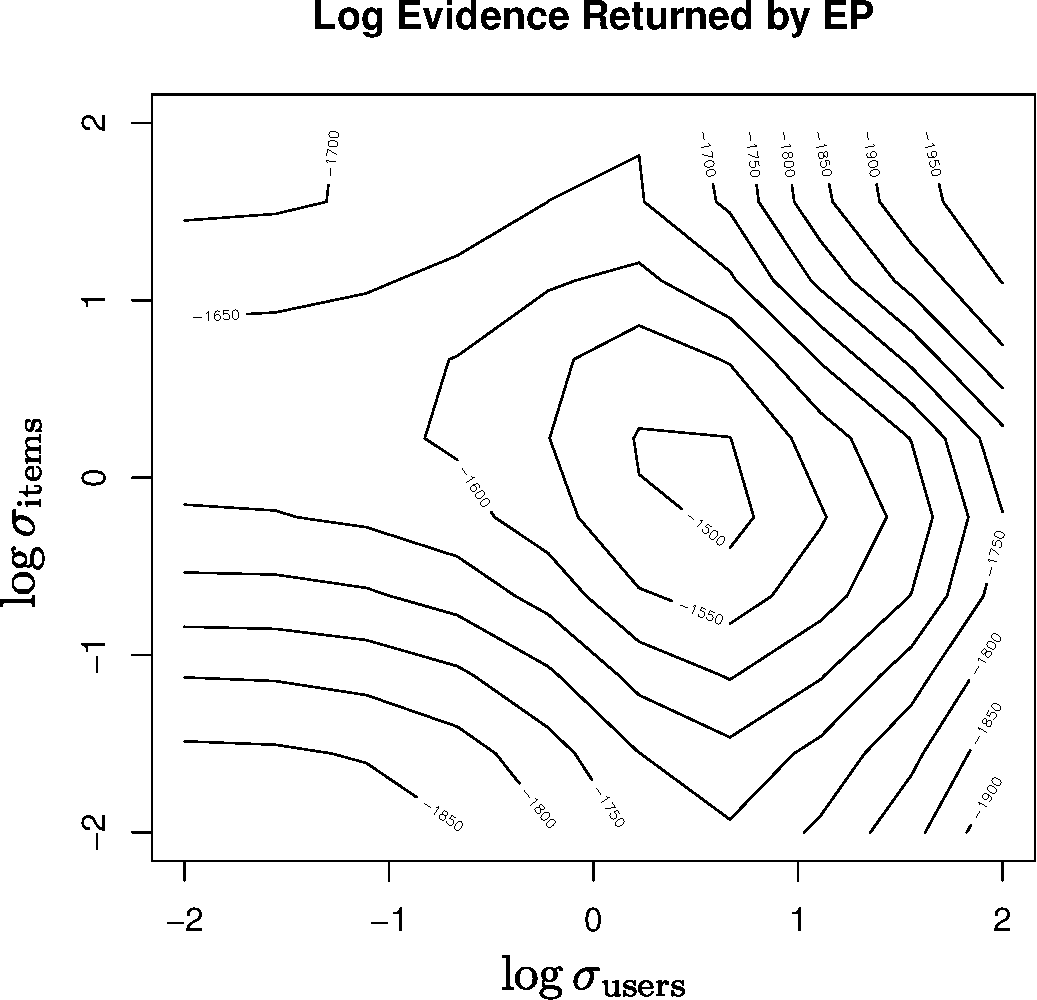
\includegraphics[scale=0.4]{figs/plotEvidence.pdf}
\caption{Logarithm of the evidence returned by EP when run on the first training set of the experiments with synthetic data.
Different values are considered for the lengthscale parameters $\sigma_\text{users}$ and $\sigma_\text{items}$.
The synthetic data are generated using $\log \sigma_\text{users} = 0$ and $\log \sigma_\text{items} = 0$.
The highest evidence returned by EP corresponds to values of $\log \sigma_\text{users}$ and
$\log \sigma_\text{items}$ close to zero.}\label{fig:experimentEvidence}
\end{figure}

\section{Tuning the kernel lengthscale}

In this section we perform an additional experiment to show that approximation of the model evidence given by EP can be used to
tune the kernel hyper-parameters in the proposed multi-task model. For this, we use the synthetic dataset
described in the main document. Figure \ref{fig:experimentEvidence} shows a contour plot of the log-evidence returned by EP 
when run on the first training set of the experiments with synthetic data and 100 users.
Different values are considered for the lengthscale parameters $\sigma_\text{users}$ and $\sigma_\text{items}$.
The synthetic data are generated using $\log \sigma_\text{users} = 0$ and $\log \sigma_\text{items} = 0$.
The highest evidence returned by EP corresponds to values of $\log \sigma_\text{users}$ and $\log \sigma_\text{items}$ close to zero.
In this experiment we are running EP using a total of 20 latent functions,
while the data are generated using only 5 latent functions.
As mentioned in the main document, the proposed multi-task model
seems to be robust to over-fitting and over-estimation of
the number of latent functions does not seem to harm predictive performance.

%\renewcommand{\arraystretch}{0.9}
\newcommand{\ic}{\hspace{0.25cm}}
\begin{table}
\centering
\caption{Average test error with 100 users.}
%\resizebox{\textwidth}{!}{
\begin{tabular}{@{\ic}l@{\ic}c@{\ic}c@{\ic}c@{\ic}c@{\ic}c@{\ic}c@{\ic}}
\hline
\textbf{Dataset} &\textbf{CPU}&\textbf{CP}&\textbf{BI}&\textbf{BO}&\textbf{SU}\\
\hline
Synthetic&\bf{0.163$\pm$0.007}&0.182$\pm$0.007&0.255$\pm$0.016&0.169$\pm$0.008&0.228$\pm$0.008\\
Sushi&0.125$\pm$0.009&\bf{0.115$\pm$0.010}&0.196$\pm$0.011&0.253$\pm$0.008&0.153$\pm$0.010\\
MovieLens&0.187$\pm$0.008&\bf{0.166$\pm$0.006}&0.205$\pm$0.009&0.314$\pm$0.007&0.223$\pm$0.008\\
Election&0.232$\pm$0.015&\bf{0.154$\pm$0.015}&\bf{0.153$\pm$0.011}&0.385$\pm$0.017&0.309$\pm$0.014\\
Jura&0.162$\pm$0.015&\bf{0.154$\pm$0.011}&0.188$\pm$0.022&0.181$\pm$0.014&0.185$\pm$0.013\\
\hline
\end{tabular} \label{tab:errorSmallDatasets}
%}
\label{tab:small}
\end{table}

\renewcommand{\ic}{\hspace{0.3cm}}
\begin{table}
\centering
\caption{Test error for each method and active learning strategy with at most 1000 users.}
\resizebox{0.79\textwidth}{!}{
\begin{tabular}{@{\ic}l@{\ic}@{\ic}c@{\ic}c@{\ic}c@{\ic}@{\ic}c@{\ic}c@{\ic}c@{\ic}@{\ic}c@{\ic}c@{\ic}c@{\ic}}
\hline
\textbf{Dataset}&\textbf{CPU-B}&\textbf{CPU-E}&\textbf{CPU-R}&
\textbf{CP-B}&\textbf{CP-E}&\textbf{CP-R}&\textbf{SU-B}&\textbf{SU-E}&\textbf{SU-R}\\\hline

Synthetic&\underline{\bf{0.135}}&\underline{\bf{0.135}}&0.139&\bf{0.153}&0.160&0.173&\bf{0.249}&0.259&0.268\\
Sushi&\bf{0.148}&0.153&0.178&\underline{\bf{0.144}}&0.151&0.176&\bf{0.179}&0.197&0.212\\
MovieLens&\bf{0.170}&0.176&0.199&\underline{\bf{0.163}}&0.170&0.195&\bf{0.225}&0.235&0.248\\
Election&0.202&\bf{0.158}&0.224& \underline{\bf{0.097}} & \underline{\bf{0.093}} &0.151&\bf{0.332}&0.346&0.338\\
Jura&\bf{0.143}&\underline{\bf{0.141}}&0.168&\underline{\bf{0.138}}&\underline{\bf{0.138}}&0.169&0.176&\bf{0.166}&0.197\\

\hline
\end{tabular}
}
\label{tab:large}
\end{table}


\begin{figure}[h!]\centering
\resizebox{\textwidth}{!}{
\begin{tabular}{ccc}
Synthetic&
Sushi&
MovieLens\\
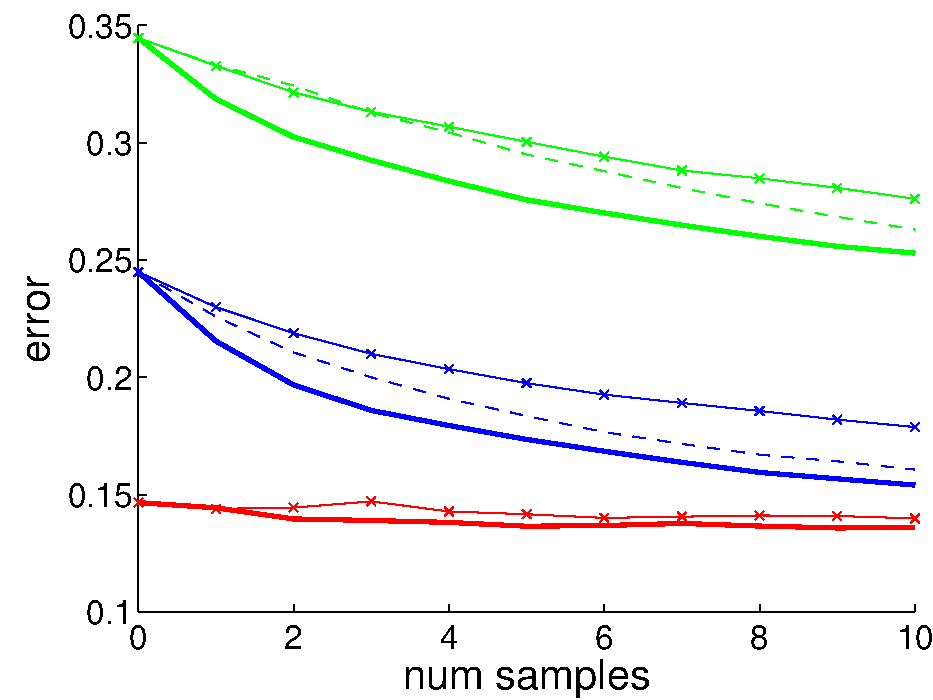
\includegraphics[scale=0.3]{figs/error_syntheticDataLargeScale.pdf}&
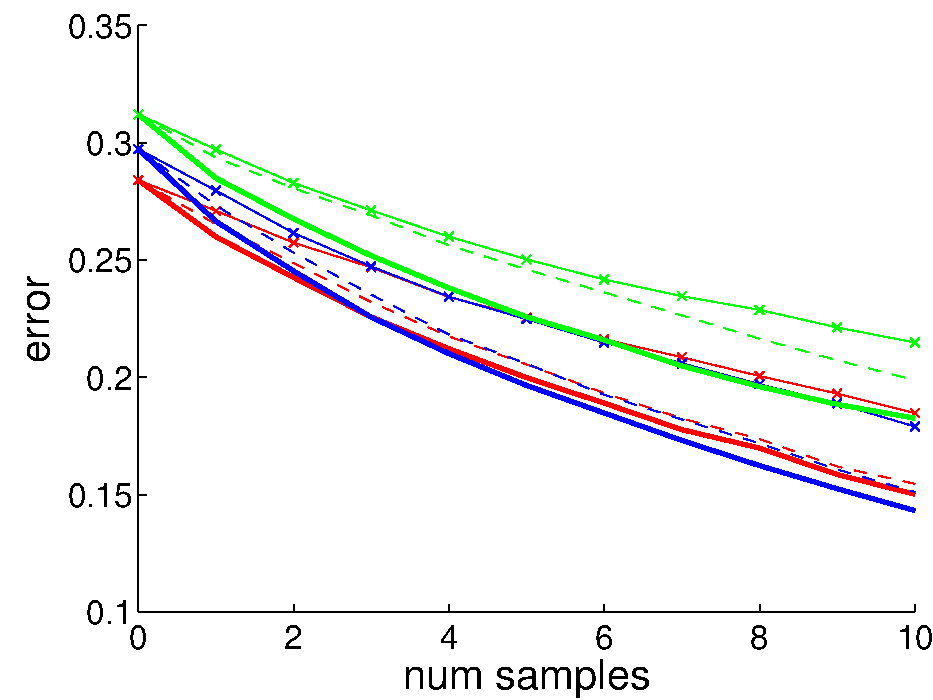
\includegraphics[scale=0.3]{figs/error_sushiDataLargeScale.pdf}&
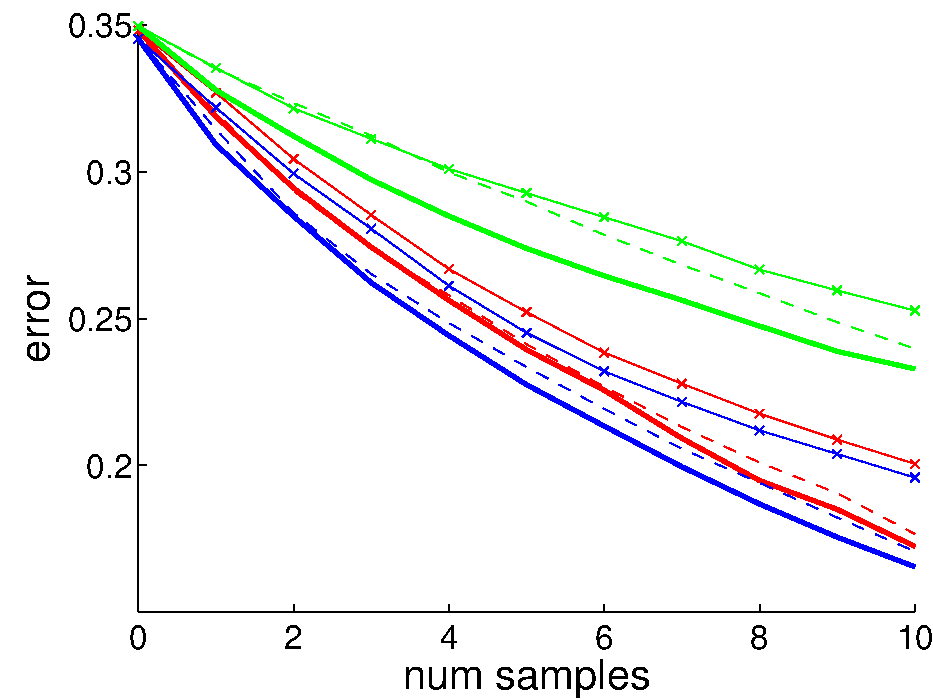
\includegraphics[scale=0.3]{figs/error_movieLensDataLargeScale.pdf}\\
Election&
Jura&
\\
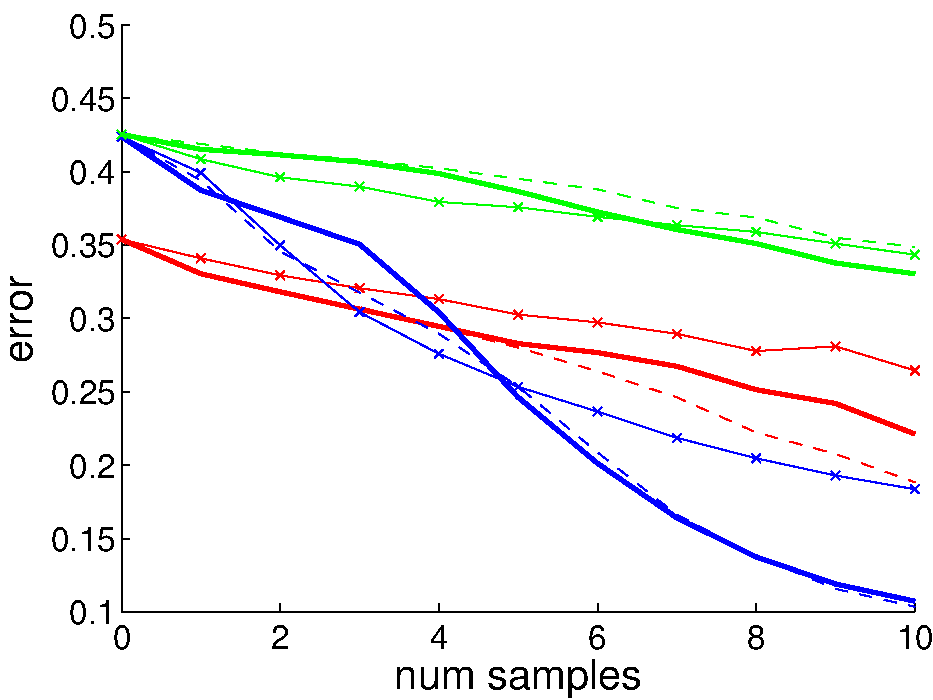
\includegraphics[scale=0.3]{figs/error_electionDataLargeScale.pdf}&
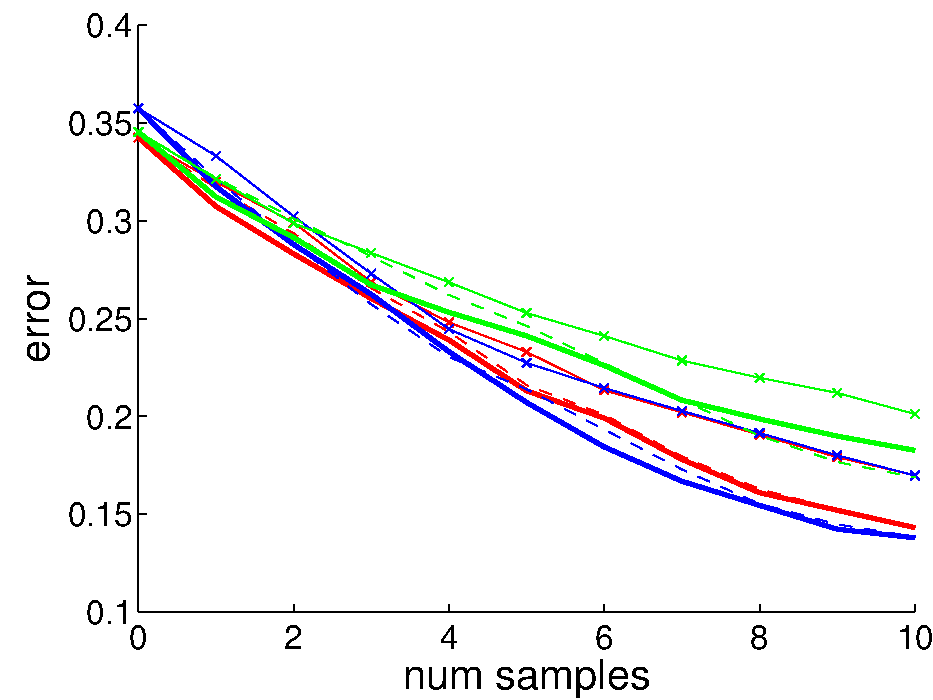
\includegraphics[scale=0.3]{figs/error_juraDataLargeScale.pdf}&
\hskip0.6cm \raisebox{0.08\height}{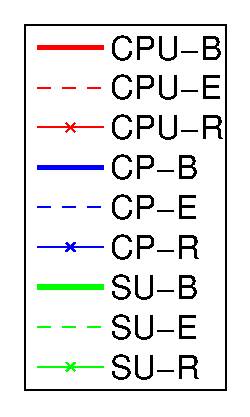
\includegraphics[scale=0.45]{figs/legend.pdf}}
\end{tabular}
}
\label{fig:learningcurves}
\caption{Average test error for CPU, CP and SU, using the strategies BALD (-B), entropy (-E) and random (-R) for active learning.}
\end{figure}

\section{Complete figures for active learning on large datasets}

Figure \ref{fig:learningcurves} shows the learning curves for all methods on all the datasets. Tables \ref{tab:small} and \ref{tab:large} are
reproductions of the tables in the results section of the main paper with information regarding the standard deviations of the results.

{
\bibliographystyle{apalike}
\bibliography{bib/bibliog}
}

\end{document}
